\documentclass[]{article}
\usepackage{lmodern}
\usepackage{amssymb,amsmath}
\usepackage{ifxetex,ifluatex}
\usepackage{fixltx2e} % provides \textsubscript
\ifnum 0\ifxetex 1\fi\ifluatex 1\fi=0 % if pdftex
  \usepackage[T1]{fontenc}
  \usepackage[utf8]{inputenc}
\else % if luatex or xelatex
  \ifxetex
    \usepackage{mathspec}
  \else
    \usepackage{fontspec}
  \fi
  \defaultfontfeatures{Ligatures=TeX,Scale=MatchLowercase}
\fi
% use upquote if available, for straight quotes in verbatim environments
\IfFileExists{upquote.sty}{\usepackage{upquote}}{}
% use microtype if available
\IfFileExists{microtype.sty}{%
\usepackage{microtype}
\UseMicrotypeSet[protrusion]{basicmath} % disable protrusion for tt fonts
}{}
\usepackage[margin=1in]{geometry}
\usepackage{hyperref}
\hypersetup{unicode=true,
            pdfborder={0 0 0},
            breaklinks=true}
\urlstyle{same}  % don't use monospace font for urls
\usepackage{natbib}
\bibliographystyle{plainnat}
\usepackage{color}
\usepackage{fancyvrb}
\newcommand{\VerbBar}{|}
\newcommand{\VERB}{\Verb[commandchars=\\\{\}]}
\DefineVerbatimEnvironment{Highlighting}{Verbatim}{commandchars=\\\{\}}
% Add ',fontsize=\small' for more characters per line
\usepackage{framed}
\definecolor{shadecolor}{RGB}{248,248,248}
\newenvironment{Shaded}{\begin{snugshade}}{\end{snugshade}}
\newcommand{\KeywordTok}[1]{\textcolor[rgb]{0.13,0.29,0.53}{\textbf{#1}}}
\newcommand{\DataTypeTok}[1]{\textcolor[rgb]{0.13,0.29,0.53}{#1}}
\newcommand{\DecValTok}[1]{\textcolor[rgb]{0.00,0.00,0.81}{#1}}
\newcommand{\BaseNTok}[1]{\textcolor[rgb]{0.00,0.00,0.81}{#1}}
\newcommand{\FloatTok}[1]{\textcolor[rgb]{0.00,0.00,0.81}{#1}}
\newcommand{\ConstantTok}[1]{\textcolor[rgb]{0.00,0.00,0.00}{#1}}
\newcommand{\CharTok}[1]{\textcolor[rgb]{0.31,0.60,0.02}{#1}}
\newcommand{\SpecialCharTok}[1]{\textcolor[rgb]{0.00,0.00,0.00}{#1}}
\newcommand{\StringTok}[1]{\textcolor[rgb]{0.31,0.60,0.02}{#1}}
\newcommand{\VerbatimStringTok}[1]{\textcolor[rgb]{0.31,0.60,0.02}{#1}}
\newcommand{\SpecialStringTok}[1]{\textcolor[rgb]{0.31,0.60,0.02}{#1}}
\newcommand{\ImportTok}[1]{#1}
\newcommand{\CommentTok}[1]{\textcolor[rgb]{0.56,0.35,0.01}{\textit{#1}}}
\newcommand{\DocumentationTok}[1]{\textcolor[rgb]{0.56,0.35,0.01}{\textbf{\textit{#1}}}}
\newcommand{\AnnotationTok}[1]{\textcolor[rgb]{0.56,0.35,0.01}{\textbf{\textit{#1}}}}
\newcommand{\CommentVarTok}[1]{\textcolor[rgb]{0.56,0.35,0.01}{\textbf{\textit{#1}}}}
\newcommand{\OtherTok}[1]{\textcolor[rgb]{0.56,0.35,0.01}{#1}}
\newcommand{\FunctionTok}[1]{\textcolor[rgb]{0.00,0.00,0.00}{#1}}
\newcommand{\VariableTok}[1]{\textcolor[rgb]{0.00,0.00,0.00}{#1}}
\newcommand{\ControlFlowTok}[1]{\textcolor[rgb]{0.13,0.29,0.53}{\textbf{#1}}}
\newcommand{\OperatorTok}[1]{\textcolor[rgb]{0.81,0.36,0.00}{\textbf{#1}}}
\newcommand{\BuiltInTok}[1]{#1}
\newcommand{\ExtensionTok}[1]{#1}
\newcommand{\PreprocessorTok}[1]{\textcolor[rgb]{0.56,0.35,0.01}{\textit{#1}}}
\newcommand{\AttributeTok}[1]{\textcolor[rgb]{0.77,0.63,0.00}{#1}}
\newcommand{\RegionMarkerTok}[1]{#1}
\newcommand{\InformationTok}[1]{\textcolor[rgb]{0.56,0.35,0.01}{\textbf{\textit{#1}}}}
\newcommand{\WarningTok}[1]{\textcolor[rgb]{0.56,0.35,0.01}{\textbf{\textit{#1}}}}
\newcommand{\AlertTok}[1]{\textcolor[rgb]{0.94,0.16,0.16}{#1}}
\newcommand{\ErrorTok}[1]{\textcolor[rgb]{0.64,0.00,0.00}{\textbf{#1}}}
\newcommand{\NormalTok}[1]{#1}
\usepackage{longtable,booktabs}
\usepackage{graphicx,grffile}
\makeatletter
\def\maxwidth{\ifdim\Gin@nat@width>\linewidth\linewidth\else\Gin@nat@width\fi}
\def\maxheight{\ifdim\Gin@nat@height>\textheight\textheight\else\Gin@nat@height\fi}
\makeatother
% Scale images if necessary, so that they will not overflow the page
% margins by default, and it is still possible to overwrite the defaults
% using explicit options in \includegraphics[width, height, ...]{}
\setkeys{Gin}{width=\maxwidth,height=\maxheight,keepaspectratio}
\IfFileExists{parskip.sty}{%
\usepackage{parskip}
}{% else
\setlength{\parindent}{0pt}
\setlength{\parskip}{6pt plus 2pt minus 1pt}
}
\setlength{\emergencystretch}{3em}  % prevent overfull lines
\providecommand{\tightlist}{%
  \setlength{\itemsep}{0pt}\setlength{\parskip}{0pt}}
\setcounter{secnumdepth}{5}
% Redefines (sub)paragraphs to behave more like sections
\ifx\paragraph\undefined\else
\let\oldparagraph\paragraph
\renewcommand{\paragraph}[1]{\oldparagraph{#1}\mbox{}}
\fi
\ifx\subparagraph\undefined\else
\let\oldsubparagraph\subparagraph
\renewcommand{\subparagraph}[1]{\oldsubparagraph{#1}\mbox{}}
\fi

%%% Use protect on footnotes to avoid problems with footnotes in titles
\let\rmarkdownfootnote\footnote%
\def\footnote{\protect\rmarkdownfootnote}

%%% Change title format to be more compact
\usepackage{titling}

% Create subtitle command for use in maketitle
\newcommand{\subtitle}[1]{
  \posttitle{
    \begin{center}\large#1\end{center}
    }
}

\setlength{\droptitle}{-2em}
  \title{}
  \pretitle{\vspace{\droptitle}}
  \posttitle{}
  \author{}
  \preauthor{}\postauthor{}
  \date{}
  \predate{}\postdate{}

\usepackage{booktabs}

\usepackage{amsthm}
\newtheorem{theorem}{Teorema}[section]
\newtheorem{lemma}{Lema}[section]
\theoremstyle{definition}
\newtheorem{definition}{Definición}[section]
\newtheorem{corollary}{Corolario}[section]
\newtheorem{proposition}{Proposición}[section]
\theoremstyle{definition}
\newtheorem{example}{Ejemplo}[section]
\theoremstyle{definition}
\newtheorem{exercise}{Ejercicio}[section]
\theoremstyle{remark}
\newtheorem*{remark}{Remarcación }
\newtheorem*{solution}{Solución}
\begin{document}

{
\setcounter{tocdepth}{2}
\tableofcontents
}
\section{Objetivos}\label{obj}

\subsection{Objetivo general}\label{objetivo-general}

Llevar a cabo a través de técnicas estadísticas un estudio del impacto
de los programas de admisión especial (PAES y PEAMA) en términos de
admisión, permanencia y graduación, en el marco de las políticas de
inclusión educativa en la Universidad Nacional de Colombia

\subsection{Objetivos específicos}\label{objetivos-especificos}

\begin{itemize}
\tightlist
\item
  Presentar una descripción del panorama general de los estudiantes de
  nuestra población de estudio con respecto a la admisión, permanecía y
  graduación.
\item
  Validar las normas aplicadas al momento de admisión para los programas
  PAES y PEAMA.
\item
  Llevar a cabo la medición del impacto de los programas PAES y PEAMA a
  los estudiantes en el momento de la admisión.
\item
  Llevar a cabo la medición del impacto de los programas que Bienestar
  ofrece a los estudiantes PAES y PEAMA durante su permanencia en las
  áreas de acompañamiento integral, gestión y fomento socioeconómico,
  salud, cultura y deportes.
\end{itemize}

\subsection{Ignorar por ahora}\label{ignorar-por-ahora}

You can label chapter and section titles using \texttt{\{\#label\}}
after them, e.g., we can reference Chapter \ref{obj}. If you do not
manually label them, there will be automatic labels anyway, e.g.,
Chapter \ref{methods}.

Figures and tables with captions will be placed in \texttt{figure} and
\texttt{table} environments, respectively.

\begin{Shaded}
\begin{Highlighting}[]
\KeywordTok{par}\NormalTok{(}\DataTypeTok{mar =} \KeywordTok{c}\NormalTok{(}\DecValTok{4}\NormalTok{, }\DecValTok{4}\NormalTok{, .}\DecValTok{1}\NormalTok{, .}\DecValTok{1}\NormalTok{))}
\KeywordTok{plot}\NormalTok{(pressure, }\DataTypeTok{type =} \StringTok{'b'}\NormalTok{, }\DataTypeTok{pch =} \DecValTok{19}\NormalTok{)}
\end{Highlighting}
\end{Shaded}

\begin{figure}

{\centering \includegraphics[width=0.8\linewidth]{bookdown_files/figure-latex/nice-fig-1} 

}

\caption{Here is a nice figure!}\label{fig:nice-fig}
\end{figure}

Reference a figure by its code chunk label with the \texttt{fig:}
prefix, e.g., see Figure \ref{fig:nice-fig}. Similarly, you can
reference tables generated from \texttt{knitr::kable()}, e.g., see Table
\ref{tab:nice-tab}.

\begin{Shaded}
\begin{Highlighting}[]
\NormalTok{knitr}\OperatorTok{::}\KeywordTok{kable}\NormalTok{(}
  \KeywordTok{head}\NormalTok{(iris, }\DecValTok{3}\NormalTok{), }\DataTypeTok{caption =} \StringTok{'Here is a nice table!'}\NormalTok{,}
  \DataTypeTok{booktabs =} \OtherTok{TRUE}
\NormalTok{)}
\end{Highlighting}
\end{Shaded}

\begin{table}

\caption{\label{tab:nice-tab}Here is a nice table!}
\centering
\begin{tabular}[t]{rrrrl}
\toprule
Sepal.Length & Sepal.Width & Petal.Length & Petal.Width & Species\\
\midrule
5.1 & 3.5 & 1.4 & 0.2 & setosa\\
4.9 & 3.0 & 1.4 & 0.2 & setosa\\
4.7 & 3.2 & 1.3 & 0.2 & setosa\\
\bottomrule
\end{tabular}
\end{table}

You can write citations, too. For example, we are using the
\textbf{bookdown} package \citep{R-bookdown} in this sample book, which
was built on top of R Markdown and \textbf{knitr} \citep{xie2015}.

\section{Marco conceptual}\label{marco}

\subsection{Análisis de correspondencias
múltiples}\label{analisis-de-correspondencias-multiples}

Como se presenta en Pardo \citep[pp.~125 - 163]{Pardo}, el análisis de
correspondencias múltiples es una herramienta estadística cuyo objetivo
es analizar asociaciones entre categorías de las variables de interés,
esto a través de métodos gráficos que permitan observar cuales
categorías de una variable son las que más afectan a las diferentes
categorías de las otras variables, además permite reducir la dimensión
de la matriz de datos de tal manera que se pueda llegar a observar las
relaciones de las categorías usando un gráfico bidimensional. Se puede
entender como un análisis de correspondencias simples aplicado a una
tabla disyuntiva completa o bien aplicado a la tabla de Burt
correspondiente teniendo en cuenta que en este caso se pierde la
información por individuo. El método, como ya se dijo, se puede entender
como la generalización de un análisis de correspondencias simple al caso
de más de dos variables categóricas de interés, pero también se puede
entender como la realización de dos diferentes análisis de componentes
principales, uno de ellos permite hacer los cálculos de una manera
relativamente sencilla y el otro ayuda a llevar a cabo la interpretación
de los ejes obtenidos, en general, esta interpretación se hace
únicamente sobre las categorías de las variables y no sobre los
individuos ya que los últimos son, en la mayoría de los casos, anónimos.
Para seleccionar el número de ejes a retener se usan dos metodologías,
la primera es elegir el número a través del histograma de valores
propios de los ejes de acuerdo a la cantidad de valores propios que se
puedan considerar diferentes, y si hay muchos valores propios similares
se considera que pertenecen a ejes ``parásitos'', es decir a ejes que no
brindan más información. La segunda metodología se conoce como el
criterio de Benzecri, dentro de los ejes cuyo valor propio sea mayor al
inverso del número de categorías dentro del análisis se recalcula las
tasas de inercia y se selecciona el número de ejes a través del
histograma de las tasas de inercia recalculadas de la misma manera que
se hizo con el histograma de valores propios. El análisis de
correspondencias múltiples permite, además, incluir la proyección de
variables que no participaron en la construcción de los ejes, a estas
variables se les conoce como suplementarias y sirve para describir las
posibles relaciones que presentan esas categorías suplementarias con las
categorías de las variables activas del análisis.

\subsection{Modelos multinomiales}\label{modelos-multinomiales}

Cuando en un problema de modelación estadística, la variable dependiente
o de respuesta es de tipo categórico nominal una de las opciones para
llevar a cabo el análisis es recurrir a modelos logit de categoría base
adecuados a respuestas de tipo nominal \citep[pp.~267]{Agresti}. Este
modelo, también conocido como modelo multinomial, es un análisis
conjunto de modelos logit binarios para cada par de categorías como se
observa en la ecuación (1):

\[\log { \left( \frac { { \pi  }_{ j } }{ { \pi  }_{ J } }  \right)  } ={ \alpha  }_{ j }+{ \beta  }_{ j }x,\quad \quad \quad j=1,\cdots ,J-1 \quad \quad(1)\]

Donde \(J\) es el número total de categórias, \(x\) es una matriz cuyas
columnas corresponden a las variables explicativas, \({ \alpha }_{ j }\)
y \({ \beta }_{ j }\) son los parámetros a estimar en el modelo y
\({ \pi }_{ j }(x)=P(Y=j|x)\) las probabilidades asociadas a cada una de
las categorías de la variable respuesta \(Y\) con
\(\sum _{ j=1 }^{ J }{ { \pi }_{ j }(x) } =1\). Nótese que se puede
hallar la asociación de cualquier par de categorías a través de la
ecuación (2):

\[\log { \left( \frac { { \pi  }_{ a } }{ { \pi  }_{ b } }  \right)  } =\log { \left( \frac { { \pi  }_{ a } }{ { \pi  }_{ J } }  \right)  } -\log { \left( \frac { { \pi  }_{ b } }{ { \pi  }_{ J } }  \right)  } \quad \quad (2)\]

Para llevar a cabo la comparación entre modelos y poder seleccionar el
más adecuado, en términos de cuáles son las variables que lo van a
conformar y de la parsimonia del modelo, se usa el AIC o criterio de
información de Akaike, el cual evalúa al modelo de acuerdo a la cercanía
entre los valores ajustados a través del modelo y los verdaderos valores
penalizando por el número de parámetros \citep[pp.~216]{Agresti} y
permite comparar el ajuste de modelos que no están anidados. Cuando se
usa el AIC el modelo que más se ajusta a los datos será aquel que tenga
menor AIC y también se usa el BIC o criterio de información bayesiano,
el cual es muy similar al AIC, pero además toma en cuenta el tamaño de
la muestra \citep[pp.~257]{Agresti}. El proceso que se lleva a cabo para
la selección del modelo se conoce como backward o eliminación hacia
atrás, y se conduce como en \citet[ pp.~214]{Agresti}, es decir se parte
del modelo más completo y se elimina un parámetro a la vez. Para llevar
a cabo la estimación de las probabilidades de respuesta a través del
modelo se aplica la fórmula (3):

\[{ \hat { \pi  }  }_{ j }(x)=\frac { exp({ \hat { \alpha  }  }_{ j }+{ \hat { \beta ' }  }_{ j }x) }{ 1+\sum _{ h=1 }^{ J-1 }{ exp({ \hat { \alpha  }  }_{ h }+{ \hat { \beta ' }  }_{ h }x) }  } \quad \quad (3)\]

Y como se observa en la ecuación (4), los parámetros se pueden
interpretar a través del logit de una probabilidad condicional:

\[\log { \left( \frac { { \pi  }_{ j } }{ { \pi  }_{ J } }  \right)  } =\log { \left( \frac { \left( \frac { { \pi  }_{ j } }{ { \pi  }_{ J }+{ \pi  }_{ j } }  \right)  }{ \left( \frac { { \pi  }_{ J } }{ { \pi  }_{ J }+{ \pi  }_{ j } }  \right)  }  \right)  } =\log { \left( \frac { \left( \frac { { \pi  }_{ j } }{ { \pi  }_{ J }+{ \pi  }_{ j } }  \right)  }{ 1-\left( \frac { { \pi  }_{ j } }{ { \pi  }_{ J }+{ \pi  }_{ j } }  \right)  }  \right)  } =logit\left( \frac { { \pi  }_{ j } }{ { \pi  }_{ J }+{ \pi  }_{ j } }  \right) \quad \quad (4)\]

\subsection{Modelos multinomiales logísticos
multinivel}\label{modelos-multinomiales-logisticos-multinivel}

Los modelos multinivel aparecen, principalmente, en aplicaciones de la
estadística para hacer análisis con respecto a la educación
\citep{Goldstein}. Surgen como una ampliación a los modelos
generalizados ya existentes, para los cuales uno de sus supuestos
básicos es la independencia de las observaciones, pero al observar que
los individuos que se están analizando se encuentran agrupados
(estudiantes dentro de salones, salones dentro de colegios, etc\ldots{})
y que dentro de los grupos los individuos, en general, son similares
pero entre grupos existen diferencias más claras, es decir, se viola el
supuesto de independencia los modelos existentes ya no son válidos en
este caso. En términos simples, el modelo multinivel hace una corrección
al problema de independencia a través de la inclusión de variables
aleatorias correspondientes a los múltiples niveles de anidación de
nuestros datos y que permiten llevar cabo estimaciones correctas de los
parámetros del modelo. Para nuestro caso el modelo de interés es de
respuesta categórica nominal, de ahí que el modelo a usar resulte un
modelo multinomial logístico multinivel \citep{Goldstein} de manera en
que se especifica en la fórmula (5):

\[\log { \left( \frac { { { \pi  }_{ j } }^{ (s) } }{ { { \pi  }_{ J } }^{ (s) } }  \right)  } ={ \alpha  }_{ j }+{ \beta  }_{ j }{ x }^{ (s) }+{ { u }_{ j } }^{ (s) },\quad \quad \quad j=1,\cdots ,J-1\quad \quad (5)\]

Donde \(J\) es el número total de categórias, x es una matriz cuyas
columnas corresponden a las variables explicativas, \({ \alpha }_{ j }\)
y \({ \beta }_{ j }\) son los parámetros a estimar en el modelo, \(s\)
es el nivel de agrupación de las observaciones y
\({ { \pi }_{ j } }^{ (s) }({ x }^{ (s) })=P(Y=j|{ x }^{ (s) },s)\) las
probabilidades asociadas a cada una de las categorías de la variable
respuesta Y en cada uno de los niveles (\(S\)),
\(\sum _{ j=1 }^{ J }{ \sum _{ s=1 }^{ S }{ { { \pi }_{ j } }^{ (s) }(x) } } =1\)
y el \({ { u }_{ j } }^{ (s) }\) es un error aleatorio asociado a cada
nivel. Se tienen como opciones la cuasi verosimilitud, la máxima
verosimilitud o los procedimientos MCMC para la estimación de los
parámetros. Pero como se presenta en \citep{HadfieldBook}:

\emph{``En el contexto de los modelos lineales generalizados mixtos
(GLMM), aquí está lo que yo observo como los pros y los contras de usar
máxima verosimilitud (restringida - REML) versus los métodos bayesianos
de Cadenas de Markov de Monte Carlo (MCMC). REML son rápidos y fáciles
de usar, mientras los métodos MCMC pueden ser lentos y más retadores
técnicamente. En particular, el reto es la especificación de una apiori
sensible, el cual no es una dificultad con REML. Sin embargo, los
resultados analíticos para GLMM no Gaussianos en general no están
disponibles y REML se basa en procedimientos que usan métodos de máxima
verosimilitud aproximada que pueden no funcionar bien. MCMC también es
una aproximación, pero la exactitud de la aproximación incrementa en la
misma medida que aumenta la longitud del análisis, siendo exactos al
límite. Adicionalmente REML usa teoría de grandes muestras para derivar
las aproximaciones de los intervalos de confianza los cuales pueden ser
muy pobres especialmente para las varianzas. Nuevamente, las medidas de
confianza de MCMC son exactas, excepto por el error de Monte Carlo, y
proveen de una manera fácil e intuitiva de obtener medidas de confianza
derivadas de las estadísticas como las razones de varianza,
correlaciones y predicciones.''}

Luego para tamaños de muestra grandes y siempre que los métodos
computacionales estén disponibles se puede acudir a métodos de
estimación REML, en los demás casos la solución será acudir a métodos de
estimación MCMC. Para más detalles sobre la estimación de parámetros de
los modelos multinivel desde la perspectiva frecuentista de los modelos
multinivel véase (Goldstein, 2010) y para la estimación de los
parámetros desde la perspectiva bayesiana véase \citep{Goldstein} y/o
\citep{HadfieldBook}. Para validar los supuestos y ajuste de los modelos
multinivel existen dos caminos a seguir y dependen de la manera en que
decidamos hacer la estimación de los parámetros de nuestro modelo. En la
primera manera, es decir, la frecuentista o REML los supuestos son: en
primera medida que los datos provengan de la distribución de
probabilidades teorizada por el modelo, pero a diferencia de los modelos
lineales generalizados usuales, los modelos multinivel no requieren la
independencia de los errores. En la segunda manera, es decir, la
bayesiana o MCMC los supuestos son: que los datos provengan de la
distribución de probabilidades teorizada por el modelo, que la
distribución a priori (que puede, o no, ser informativa) conjugue con la
función de máxima verosimilitud de los datos, además se debe verificar
que las cadenas de Márkov converjan para la estimación de los
parámetros. Al llevar a cabo las verificaciones anteriormente descritas
y apropiadas al método usado para la estimación entonces se garantiza
que nuestro modelo ha sido validado y que el mismo se ha ajustado a
nuestros datos.

\subsection{Software estadístico R:}\label{software-estadistico-r}

R es un leguaje y ambiente de computación estadístico de código libre
(GNU project) construido para dar sentido y valor agregado a los datos.
R provee de una muy amplia variedad de herramientas estadísticas la cual
es alimentada por su activa y creciente comunidad de colaboradores y
usuarios. RStudio es una IDE (entorno de desarrollo integrado) para R,
la comunidad de desarrolladores de RStudio inspirados por las
innovaciones de los usuarios de R en las ciencias, educación e industria
desarrollaron gran cantidad de herramientas, la mayoría libres, que
permite dar gran valor añadido a los datos (dashboards, htmlwidgets,
libros, etc\ldots{}) y para que los equipos de trabajo puedan promover y
compartir el trabajo posicionando a R como el lenguaje estadístico, de
inteligencia de negocios y de ciencia de datos más poderoso, innovador y
de mayor crecimiento en el mundo. Entre la gran variedad de librerías
que posee R describiremos a continuación aquellas que fueron utilizadas
en el desarrollo del proyecto. \textbf{Referencias:} \citep{r1},
\citep{wikiR}, \citep{wikiRStudio}, \citep{rstudio1}, \citep{rstudio2}.

\subsubsection{Librería tidyverse:}\label{libreria-tidyverse}

Es una colección de paquetes de R diseñados para ciencia de datos. Todos
los paquetes comparten una filosofía de diseño subyacente, gramática y
estructuras de datos. Contiene ggplot2 la cual es una librería poderosa
para hacer gráficos estáticos por capas, dplyr la cual sirve para la
manipulación de datos, tidyr la cual ayuda a depurar las bases de datos,
readr para la lectura de datos rectangulares, readxl para la lectura de
archivos .xls y .xlsx, purrr la cual permite hacer programación
funcional, tibble la cual es una manera moderna de pensar las
estructuras de datos, stringr la cual se encarga de que el trabajo con
caracteres (strings) sea lo más sencillo posible, forcats la cual
permite solucionar problemas frecuentes con la manipulación de factores,
entre otros muchos paquetes. \textbf{Referencias:} \citep{tidyverse}

\subsubsection{Librería Factoclass:}\label{libreria-factoclass}

Como lo describe dos de sus autores Campo Elías Pardo (profesor asociado
del Departamento de Estadística de la Universidad Nacional de Colombia)
y Pedro César del Campo (Estadístico de la Universidad Nacional de
Colombia) en \citep{Pardo2007}, el paquete se implementó con la
finalidad de llevar a cabo exploración multivariada de datos de acuerdo
con las estrategias descritas en \citep{Lebart} . \textbf{Referencias:}
\citep{Factoclass}

\subsubsection{Librería lme4:}\label{libreria-lme4}

Es una librería construida para el ajuste de modelos lineales de efectos
mixtos y modelos lineales generalizados de efectos mixtos desde un
enfoque de máxima verosimilitud restringida. \textbf{Referencias:}
\citep{lme4}, \citep{Bates}

\subsubsection{Librería MCMCglmm:}\label{libreria-mcmcglmm}

Es una librería de R la cual tiene como objetivo ajustar modelos
lineales generalizados mixtos con un enfoque bayesiano a través del uso
de Cadenas de Markov Monte Carlo (MCMC). \textbf{Referencias:}
\citep{MCMCglmm}, \citep{HadfieldBook}, \citep{HadfieldCourseNotes}.

\section{Metodología}\label{metodologuxeda}

La metodología llevada a cabo se divide en hacer análisis para los
estudiantes PAES y para los estudiantes PEAMA, que ingresaron en la
cohorte 2011-01, por separado. La metodología en ambos casos es la misma
y consta de los siguientes pasos:

\begin{enumerate}
\def\labelenumi{\arabic{enumi}.}
\tightlist
\item
  Construcción descriptiva del panorama de admisión de cada una de las
  dos poblaciones (PEAMA y PAES).
\item
  Revisión de la normatividad existente al ingreso de los dos grupos y
  su posterior validación.
\item
  Construcción de un único modelo binomial logit multinivel global de
  admisión.
\item
  Construcción de análisis de correspondencias múltiples para las
  variables incluidas en la permanencia y graduación que permita
  comprender cuales van a ser incluidas en el modelo para cada uno de
  los dos grupos de estudiantes (PAES y PEAMA).
\item
  Construcción de dos modelos multinomiales logit multinivel para cada
  uno de los grupos estudiantiles (PAES y PEAMA) que permita analizar
  permanencia y egreso de los estudiantes.
\end{enumerate}

\section{Admisión PAES}\label{admision-paes}

En este capítulo se presenta una descripción del panorama general de
admisión de los estudiantes PAES de la cohorte 2011-01.

En primer lugar se observa cuales fueron los programas PAES por los que
los aspirantes fueron admitidos:

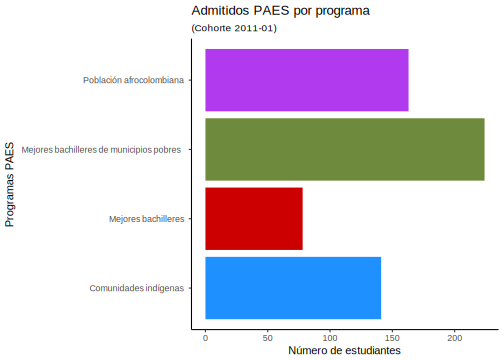
\includegraphics{bookdown_files/figure-latex/unnamed-chunk-2-1.pdf}

Observamos que la mayor parte entran por el programa \emph{mejores
bachilleres de municipios pobres} con 224 admitidos, seguido por las
\emph{poblaciones negras, afrocolombianas, palenqueras y raizales} con
163 admitidos, en tercer lugar las \emph{comunidades indígenas} con 141
admitidos y finalmente los \emph{mejores bachilleres} en último lugar
con 78 admitidos.

\subsection{Sexo de los admitidos}\label{sexo-de-los-admitidos}

Donde se encuentra que aproximadamente la tercera parte de la población
admitida como estudiantes PAES es mujer y que los restantes son hombres.
Se observa que esto ocurre además para todos los PAES de manera global y
desagregado por los programas de admisión.

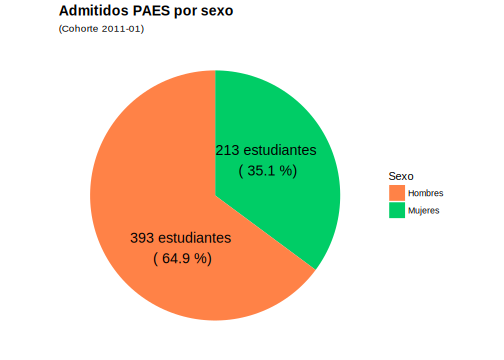
\includegraphics{bookdown_files/figure-latex/unnamed-chunk-3-1.pdf}
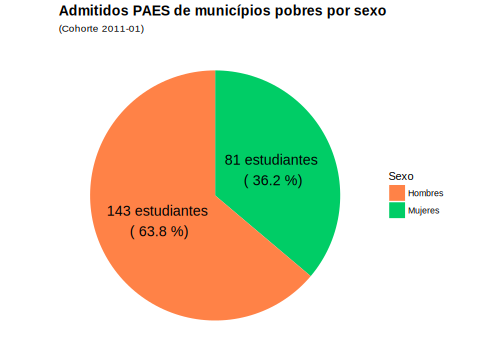
\includegraphics{bookdown_files/figure-latex/unnamed-chunk-3-2.pdf}
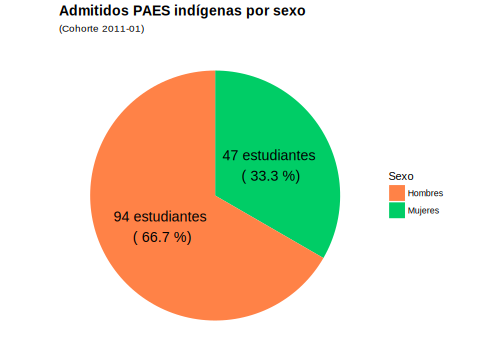
\includegraphics{bookdown_files/figure-latex/unnamed-chunk-3-3.pdf}
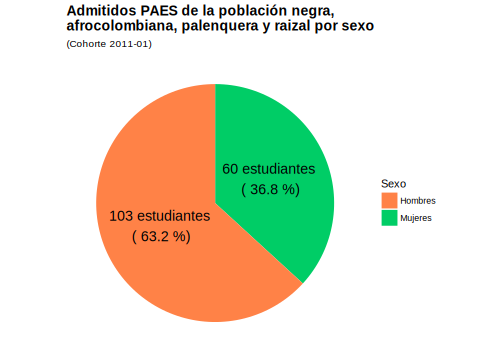
\includegraphics{bookdown_files/figure-latex/unnamed-chunk-3-4.pdf}
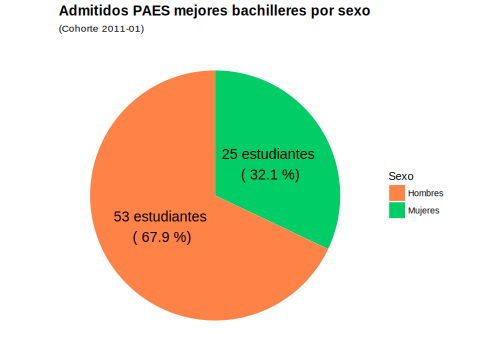
\includegraphics{bookdown_files/figure-latex/unnamed-chunk-3-5.pdf}

\subsection{Edad de los admitidos}\label{edad-de-los-admitidos}

Se haya que los estudiantes PAES admitidos tienen edades que se acumulan
principalmente entre los 16 y los 21 años siendo similar en todos los
grupos, se observa además que los grupos indígenas son los que tienen
más estudiantes en grupos de más edad (superiores a los 25 años).

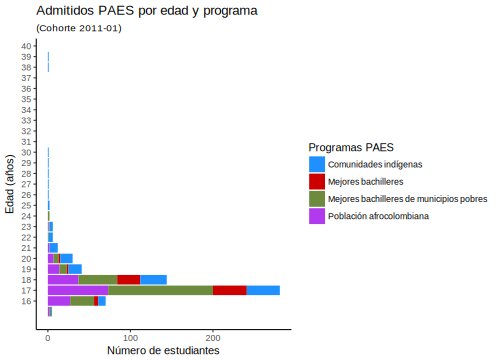
\includegraphics{bookdown_files/figure-latex/unnamed-chunk-4-1.pdf}
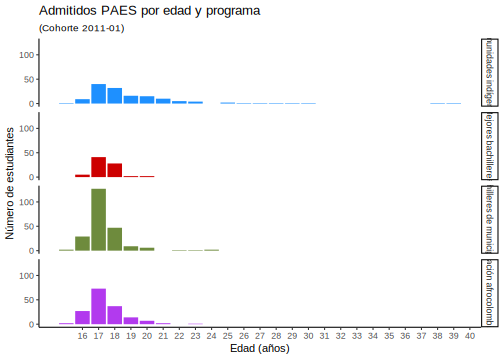
\includegraphics{bookdown_files/figure-latex/unnamed-chunk-4-2.pdf}
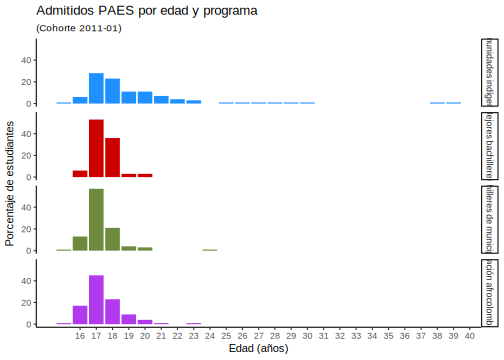
\includegraphics{bookdown_files/figure-latex/unnamed-chunk-4-3.pdf}

\subsection{Sede andina de los
admitidos}\label{sede-andina-de-los-admitidos}

Se observa que aproximadamente la mitad de los estudiantes PAES son
admitidos a la sede Bogotá, aproximadamente una cuarta parte son
admitidos a la sede Medellín y luego son admitidos a la sede Palmira y
finalmente a la sede Manizales, en cada caso con aproximadamente el 12\%
en cada caso.

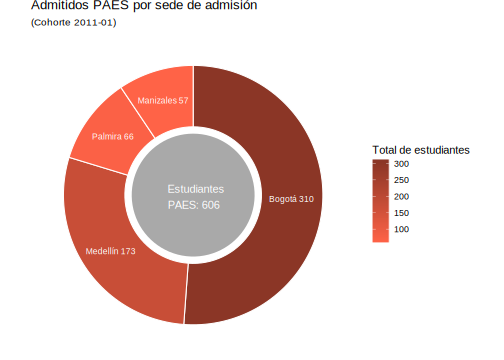
\includegraphics{bookdown_files/figure-latex/unnamed-chunk-5-1.pdf}

\subsection{Sede andina y programa de los
admitidos}\label{sede-andina-y-programa-de-los-admitidos}

Se presenta a continuación los admitidos PAES por sede y por programa.
Se encuentra que el máximo número de admitidos en algún programa es de
15 estudiantes y ocurre para el programa curricular de Administración de
Empresas de la sede de Palmira. Observamos que las cinco carreras con
más admitidos son: Palmira Administración de Empresas (15 estudiantes),
Bogotá Ingeniería Eléctrica (14 estudiantes), Bogotá Química (13
estudiantes), Palmira Ingeniería Agroindustrial y Palmira Ingeniería
Ambiental (ambas con 12 estudiantes).

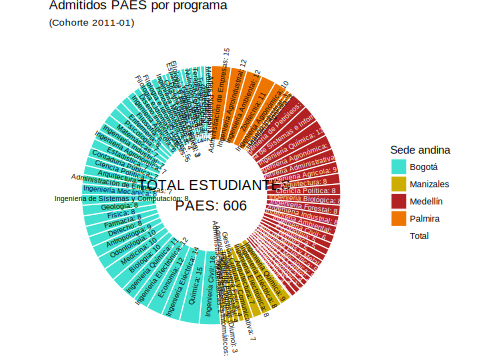
\includegraphics{bookdown_files/figure-latex/unnamed-chunk-6-1.pdf}

\subsection{Sede andina y facultad de los
admitidos}\label{sede-andina-y-facultad-de-los-admitidos}

Se hace la misma descripción anterior a los estudiantes PAES pero por
sede y facultad encontrándose que la mayor facultad con estudiantes
admitidos es la de Minas en Medellín (74 estudiantes), seguida por
Ingeniería Bogotá (65 estudiantes), Ciencias Bogotá (52 estudiantes),
Ingeniería y Administración Palmira (45 estudiantes), Ciencias Humanas
Bogotá (44 estudiantes) e Ingeniería y Administración Manizales (37
estudiantes), donde se observa un gran interés principalmente por la
ingeniería en los admitidos PAES.

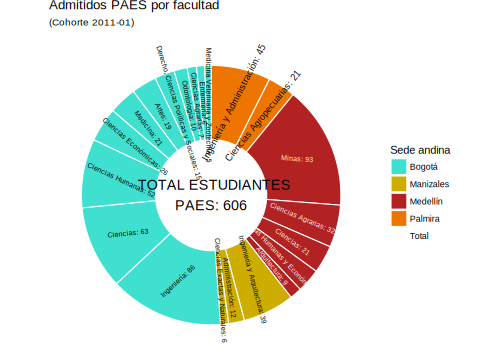
\includegraphics{bookdown_files/figure-latex/unnamed-chunk-7-1.pdf}

\subsection{Estrato socioeconómico de los
admitidos}\label{estrato-socioeconomico-de-los-admitidos}

Se hace la misma descripción anterior a los estudiantes PAES pero por
sede y facultad encontrándose que la mayor facultad con estudiantes
admitidos es la de Minas en Medellín (74 estudiantes), seguida por
Ingeniería Bogotá (65 estudiantes), Ciencias Bogotá (52 estudiantes),
Ingeniería y Administración Palmira (45 estudiantes), Ciencias Humanas
Bogotá (44 estudiantes) e Ingeniería y Administración Manizales (37
estudiantes), donde se observa un gran interés principalmente por la
ingeniería en los admitidos PAES.

\subsubsection{Estrato agrupado:}\label{estrato-agrupado}

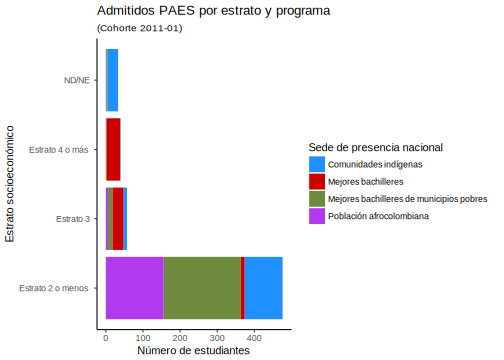
\includegraphics{bookdown_files/figure-latex/unnamed-chunk-8-1.pdf}
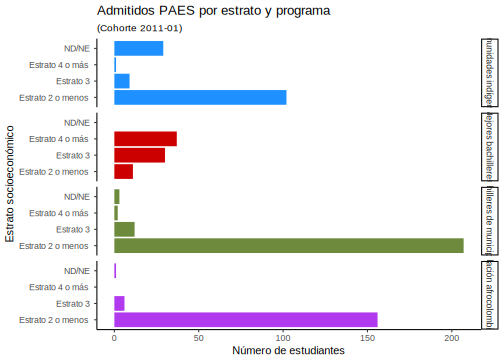
\includegraphics{bookdown_files/figure-latex/unnamed-chunk-8-2.pdf}
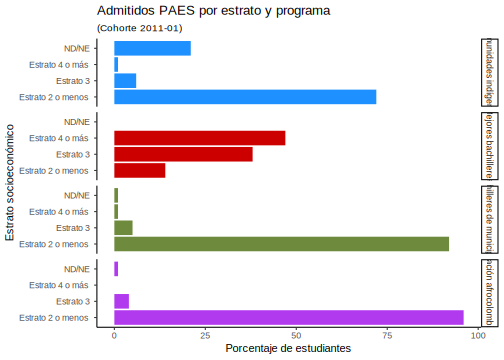
\includegraphics{bookdown_files/figure-latex/unnamed-chunk-8-3.pdf}

\subsubsection{Estrato original:}\label{estrato-original}

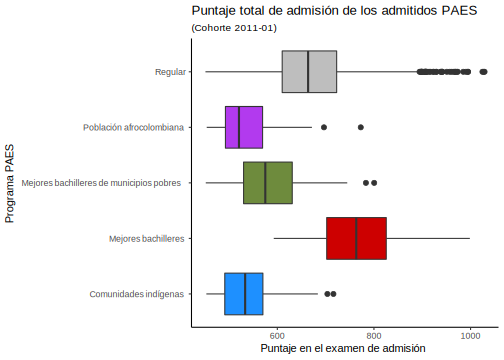
\includegraphics{bookdown_files/figure-latex/unnamed-chunk-9-1.pdf}
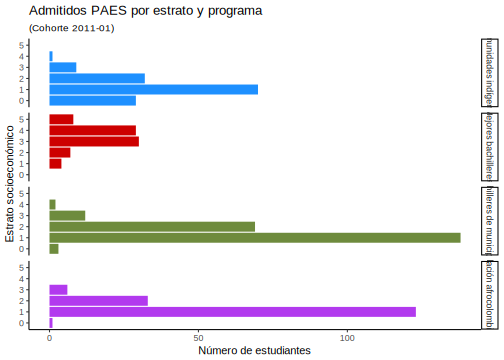
\includegraphics{bookdown_files/figure-latex/unnamed-chunk-9-2.pdf}
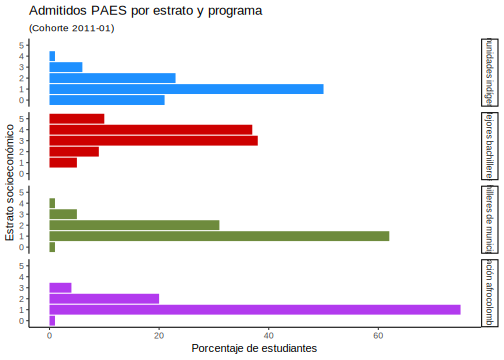
\includegraphics{bookdown_files/figure-latex/unnamed-chunk-9-3.pdf}

\subsection{Puntaje en examen de
admisión}\label{puntaje-en-examen-de-admision}

Se observa que los mayores puntajes de admisión los presentan los
estudiantes PAES correspondientes a los mejores bachilleres de
municipios pobres (con una mediana de 575,1268), seguido por los PAES
indigenas (mediana de 533.4272) y finalmente los PAES afrocolombianos,
palenqueros y raizales (mediana de 520.6273). Se observa además (en
rojo) el puntaje de admisión del último admitido de manera regular y se
encuentra que los estudiantes PAES tienen puntajes de admisión que son
iguales o superiores a ese puntaje (451,2525).

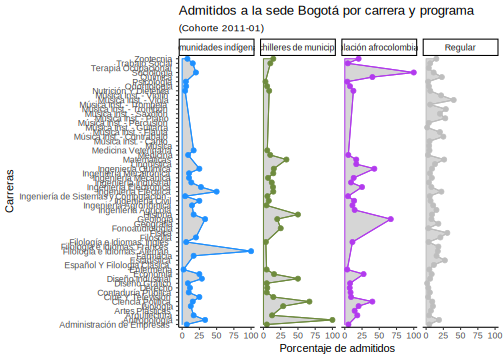
\includegraphics{bookdown_files/figure-latex/unnamed-chunk-10-1.pdf}

\subsection{Porcentaje de admitidos v.s. total de
aspirantes}\label{porcentaje-de-admitidos-v.s.-total-de-aspirantes}

Si comparamos a los admitidos con los aspirantes para cada programa
curricular y programa PAES obtenemos el porcentaje de admisión, que
también se puede ver como un índice de absorción específico. En el caso
de la sede Bogotá y de la sede Manizales se tiene que los porcentajes de
admisión dentro de los programas especiales de admisión son mayores
comparados con los porcentajes de admisión para los admitidos regulares,
excepto por unos pocos casos.

No ocurre lo mismo para las sedes Medellín y Palmira, en el primero se
tienen muchos casos donde la porcentaje de admitidos es mayor en los
programas PAES comparados con los regulares, así mismo se tienen muchos
casos donde el porcentaje de admitidos regulares es mayor comparado con
el de admitidos PAES por programa. En el caso de la sede Palmira se
observa que en la mayoría de casos los admitidos por programa tienen una
mayor proporción comparados con la proporción que existe dentro de cada
uno de los programas PAES.

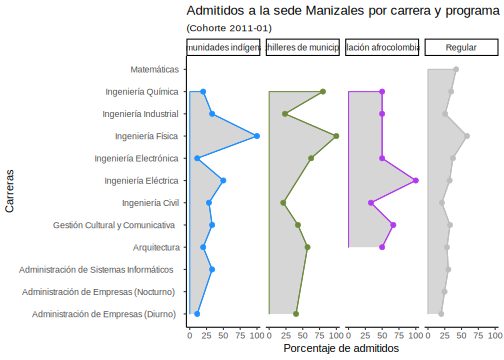
\includegraphics{bookdown_files/figure-latex/unnamed-chunk-11-1.pdf}
\includegraphics{bookdown_files/figure-latex/unnamed-chunk-11-2.pdf}
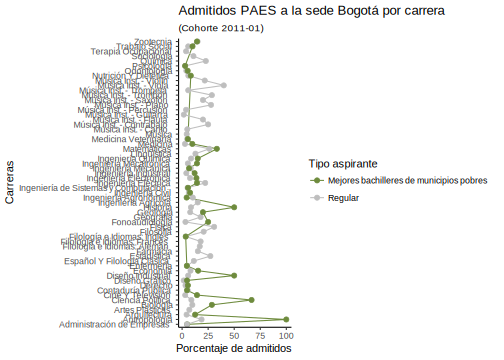
\includegraphics{bookdown_files/figure-latex/unnamed-chunk-11-3.pdf}
\includegraphics{bookdown_files/figure-latex/unnamed-chunk-11-4.pdf}

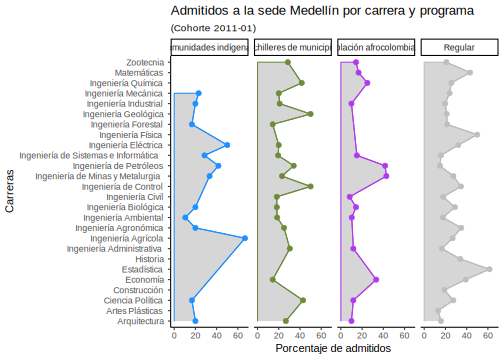
\includegraphics{bookdown_files/figure-latex/unnamed-chunk-12-1.pdf}
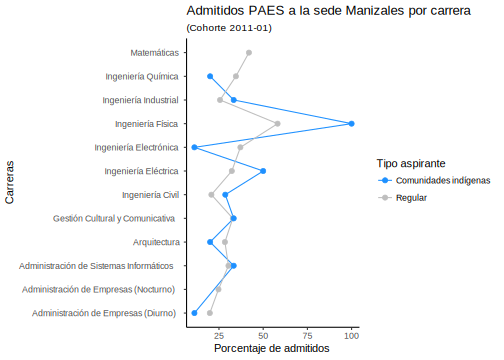
\includegraphics{bookdown_files/figure-latex/unnamed-chunk-12-2.pdf}
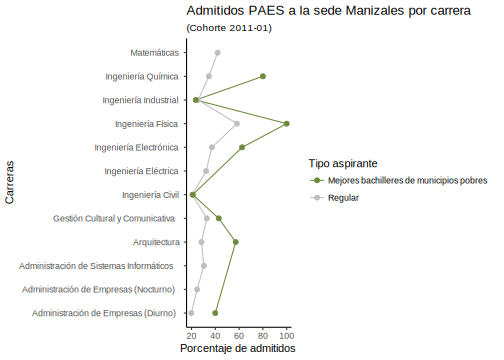
\includegraphics{bookdown_files/figure-latex/unnamed-chunk-12-3.pdf}
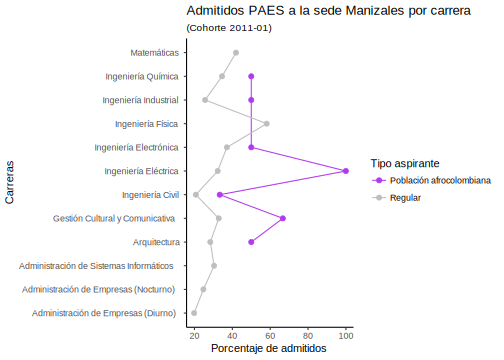
\includegraphics{bookdown_files/figure-latex/unnamed-chunk-12-4.pdf}

\includegraphics{bookdown_files/figure-latex/unnamed-chunk-13-1.pdf}
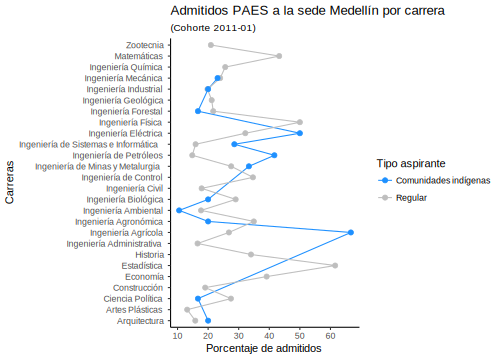
\includegraphics{bookdown_files/figure-latex/unnamed-chunk-13-2.pdf}
\includegraphics{bookdown_files/figure-latex/unnamed-chunk-13-3.pdf}
\includegraphics{bookdown_files/figure-latex/unnamed-chunk-13-4.pdf}

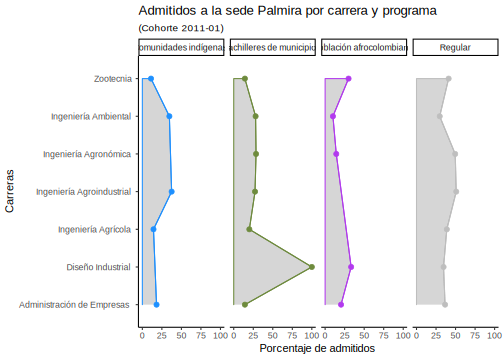
\includegraphics{bookdown_files/figure-latex/unnamed-chunk-14-1.pdf}
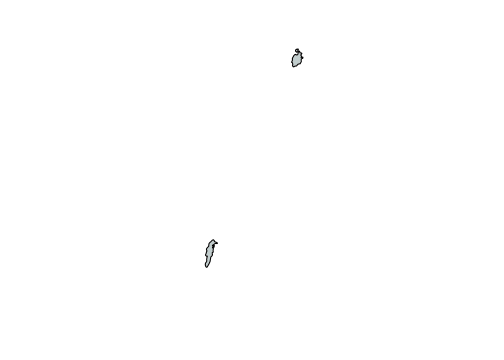
\includegraphics{bookdown_files/figure-latex/unnamed-chunk-14-2.pdf}
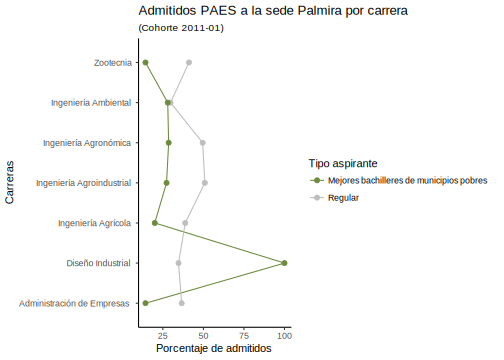
\includegraphics{bookdown_files/figure-latex/unnamed-chunk-14-3.pdf}
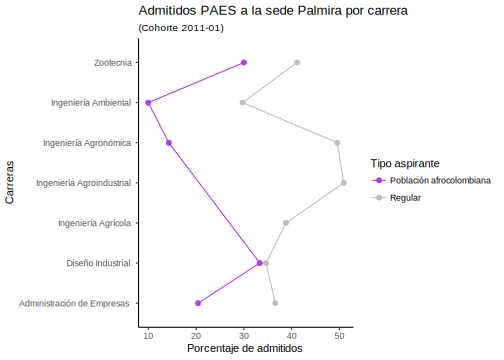
\includegraphics{bookdown_files/figure-latex/unnamed-chunk-14-4.pdf}

\subsection{Admitidos PAES por município de
residencia}\label{admitidos-paes-por-municipio-de-residencia}

\subsubsection{Todos los admitidos PAES}\label{todos-los-admitidos-paes}

\includegraphics{bookdown_files/figure-latex/unnamed-chunk-15-1.pdf}
\includegraphics{bookdown_files/figure-latex/unnamed-chunk-15-2.pdf}

\subsubsection{Admitidos PAES de las comunidades
indígenas}\label{admitidos-paes-de-las-comunidades-indigenas}

\includegraphics{bookdown_files/figure-latex/unnamed-chunk-16-1.pdf}

\subsubsection{Admitidos PAES de los mejores
bachilleres}\label{admitidos-paes-de-los-mejores-bachilleres}

\includegraphics{bookdown_files/figure-latex/unnamed-chunk-17-1.pdf}

\subsubsection{Admitidos PAES de los mejores bachilleres de municipios
pobres}\label{admitidos-paes-de-los-mejores-bachilleres-de-municipios-pobres}

\includegraphics{bookdown_files/figure-latex/unnamed-chunk-18-1.pdf}

\subsubsection{Admitidos PAES de las poblaciones
afrocolombianas}\label{admitidos-paes-de-las-poblaciones-afrocolombianas}

\includegraphics{bookdown_files/figure-latex/unnamed-chunk-19-1.pdf}

\subsection{Admitidos PAES por departamento de
residencia}\label{admitidos-paes-por-departamento-de-residencia}

\subsubsection{Todos los admitidos
PAES}\label{todos-los-admitidos-paes-1}

\includegraphics{bookdown_files/figure-latex/unnamed-chunk-20-1.pdf}
\includegraphics{bookdown_files/figure-latex/unnamed-chunk-20-2.pdf}

\subsubsection{Admitidos PAES de las comunidades
indígenas}\label{admitidos-paes-de-las-comunidades-indigenas-1}

\includegraphics{bookdown_files/figure-latex/unnamed-chunk-21-1.pdf}

\subsubsection{Admitidos PAES de los mejores
bachilleres}\label{admitidos-paes-de-los-mejores-bachilleres-1}

\includegraphics{bookdown_files/figure-latex/unnamed-chunk-22-1.pdf}

\subsubsection{Admitidos PAES de los mejores bachilleres de municipios
pobres}\label{admitidos-paes-de-los-mejores-bachilleres-de-municipios-pobres-1}

\includegraphics{bookdown_files/figure-latex/unnamed-chunk-23-1.pdf}

\subsubsection{Admitidos PAES de las poblaciones
afrocolombianas}\label{admitidos-paes-de-las-poblaciones-afrocolombianas-1}

\includegraphics{bookdown_files/figure-latex/unnamed-chunk-24-1.pdf}

\section{Admisión PEAMA}\label{admision-peama}

En este capítulo se presenta una descripción del panorama general de
admisión de los estudiantes PEAMA de la cohorte 2011-01.

En primer lugar se observa cuales fueron los programas PEAMA por los que
los aspirantes fueron admitidos y que corresponden a la sede de
presencia nacional a la cual fueron admitidos:

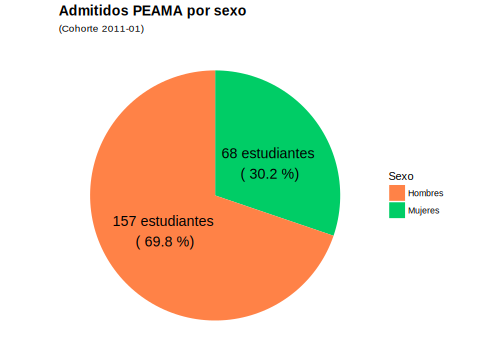
\includegraphics{bookdown_files/figure-latex/unnamed-chunk-26-1.pdf}

Observamos que la mayor parte entran por la \emph{Sede Orinoquia} con
102 admitidos, seguido por la \emph{Sede Amazonía} con 83 admitidos y en
tercer lugar la \emph{Sede Caribe} con 40 admitidos.

\subsection{Sexo de los admitidos}\label{sexo-de-los-admitidos-1}

\includegraphics{bookdown_files/figure-latex/unnamed-chunk-27-1.pdf}
\includegraphics{bookdown_files/figure-latex/unnamed-chunk-27-2.pdf}
\includegraphics{bookdown_files/figure-latex/unnamed-chunk-27-3.pdf}
\includegraphics{bookdown_files/figure-latex/unnamed-chunk-27-4.pdf}

\subsection{Edad de los admitidos}\label{edad-de-los-admitidos-1}

\includegraphics{bookdown_files/figure-latex/unnamed-chunk-28-1.pdf}
\includegraphics{bookdown_files/figure-latex/unnamed-chunk-28-2.pdf}
\includegraphics{bookdown_files/figure-latex/unnamed-chunk-28-3.pdf}

\subsection{Sede andina de admisión}\label{sede-andina-de-admision}

\includegraphics{bookdown_files/figure-latex/unnamed-chunk-29-1.pdf}

\subsection{Sedes andinas de admisión y sede de presencia
nacional}\label{sedes-andinas-de-admision-y-sede-de-presencia-nacional}

\includegraphics{bookdown_files/figure-latex/unnamed-chunk-30-1.pdf}

\subsection{Programa de admisión}\label{programa-de-admision}

\includegraphics{bookdown_files/figure-latex/unnamed-chunk-31-1.pdf}

\subsection{Estrato de los admitidos}\label{estrato-de-los-admitidos}

\includegraphics{bookdown_files/figure-latex/unnamed-chunk-32-1.pdf}
\includegraphics{bookdown_files/figure-latex/unnamed-chunk-32-2.pdf}
\includegraphics{bookdown_files/figure-latex/unnamed-chunk-32-3.pdf}

\subsection{Puntaje total de admisión}\label{puntaje-total-de-admision}

\includegraphics{bookdown_files/figure-latex/unnamed-chunk-33-1.pdf}

\subsection{Admitidos PEAMA por
municipio}\label{admitidos-peama-por-municipio}

\subsubsection{Todos los admitidos
PEAMA}\label{todos-los-admitidos-peama}

\includegraphics{bookdown_files/figure-latex/unnamed-chunk-34-1.pdf}
\includegraphics{bookdown_files/figure-latex/unnamed-chunk-34-2.pdf}

\subsubsection{Admitidos PEAMA Amazonia}\label{admitidos-peama-amazonia}

\includegraphics{bookdown_files/figure-latex/unnamed-chunk-35-1.pdf}
\includegraphics{bookdown_files/figure-latex/unnamed-chunk-35-2.pdf}

\subsubsection{Admitidos PEAMA Caribe}\label{admitidos-peama-caribe}

\includegraphics{bookdown_files/figure-latex/unnamed-chunk-36-1.pdf}
\includegraphics{bookdown_files/figure-latex/unnamed-chunk-36-2.pdf}

\subsubsection{Admitidos PEAMA
Orinoquía}\label{admitidos-peama-orinoquia}

\includegraphics{bookdown_files/figure-latex/unnamed-chunk-37-1.pdf}
\includegraphics{bookdown_files/figure-latex/unnamed-chunk-37-2.pdf}

\subsection{Admitidos PEAMA por
departamento}\label{admitidos-peama-por-departamento}

\subsubsection{Todos los admitidos
PEAMA}\label{todos-los-admitidos-peama-1}

\includegraphics{bookdown_files/figure-latex/unnamed-chunk-38-1.pdf}
\includegraphics{bookdown_files/figure-latex/unnamed-chunk-38-2.pdf}

\subsubsection{Admitidos PEAMA
Amazonia}\label{admitidos-peama-amazonia-1}

\includegraphics{bookdown_files/figure-latex/unnamed-chunk-39-1.pdf}
\includegraphics{bookdown_files/figure-latex/unnamed-chunk-39-2.pdf}

\subsubsection{Admitidos PEAMA Caribe}\label{admitidos-peama-caribe-1}

\includegraphics{bookdown_files/figure-latex/unnamed-chunk-40-1.pdf}
\includegraphics{bookdown_files/figure-latex/unnamed-chunk-40-2.pdf}

\subsubsection{Admitidos PEAMA
Orinoquía}\label{admitidos-peama-orinoquia-1}

\includegraphics{bookdown_files/figure-latex/unnamed-chunk-41-1.pdf}
\includegraphics{bookdown_files/figure-latex/unnamed-chunk-41-2.pdf}

\section{Normatividad}\label{normatividad}

Una de las mediciones fundamentales en la evaluación del impacto de los
programas PAES y PEAMA es hacer una validación de la normatividad
vigente y aplicable para la cohorte 2011-01, esto debido a que la
normatividad refleja que las zonas de impacto de los programas sean las
realmente escaladas, que se pertenezca a las poblaciones a quien va
realmente dirigida y que se les esten dando las oportunidades que estan
reglamentadas por ley y que aportan a la inclusión educativa en la
Universidad Nacional de Colombia:

\begin{table}

\caption{\label{tab:unnamed-chunk-43}Normatividad vigente y aplicable para la cohorte de estudio}
\centering
\begin{tabular}[t]{lrrlll}
\toprule
Tipo & N° & Fecha & Tema & Entidad Emisora o País & Interna o Externa\\
\midrule
Acuerdo & 22 & 1986 & Por el cual se dictan disposiciones acerca del ingreso a la Universidad de integrantes de comunidades indígenas. & Consejo Superior Universitario & Interna\\
Acuerdo & 93 & 1989 & Por el cual se crea el programa de admisión para mejores bachilleres de municipios pobres. & Consejo Superior Universitario & Interna\\
Acuerdo & 30 & 1990 & Por el cual se crea el programa de Mejores Bachilleres. & Consejo Superior Universitario & Interna\\
Acuerdo & 121 & 1991 & Por el cual se autoriza la reducción de la carga académica obligatoria a los estudiantes admitidos mediante los Acuerdos Nos. 22 de 1986 y 93 de 1989 o programas especiales. & Consejo Superior Universitario & Interna\\
Acuerdo & 3 & 1995 & Por el cual se establecen las políticas de Bienestar Universitario. & Consejo de Educación Superior (CESU) & Externa\\
\addlinespace
Acuerdo & 18 & 1999 & Por el cual se modifica el Acuerdo No. 22 de 1986, programa especial para la admisión Bachilleres miembros de Comunidades Indígenas. & Consejo Superior Universitario & Interna\\
Acuerdo & 25 & 2007 & Por se adopta el Programa Especial de Admisión y Movilidad Académica para las Sedes de Presencia Nacional. & Consejo Superior Universitario & Interna\\
Resolución & 1302 & 2007 & Por la cual se reglamenta el Programa Especial de Admisión y Movilidad Académica y se dictan algunas disposiciones para su implementación en la Sede Orinoquia de la Universidad Nacional de Colombia & Rectoria & Interna\\
Resolución & 16 & 2008 & Por lo cual se reglamenta el Programa Especial de Admisión y Movilidad Académica y se dictan algunas disposiciones para su implementación en la sede Caribe de la Universidad Nacional de Colombia & Rectoria & Interna\\
Resolución & 125 & 2008 & Por lo cual se reglamenta el Programa Especial de Admisión y Movilidad Académica y se dictan algunas disposiciones para su implementación en la sede Amazonia de la Universidad Nacional de Colombia & Rectoria & Interna\\
\addlinespace
Resolución & 1055 & 2008 & Por la cual se complementa la reglamentación del Programa Especial de Admisión y Movilidad Académica y se dictan algunas disposiciones para su implementación en las Sedes de Presencia Nacional de la Universidad Nacional de Colombia & Rectoria & Interna\\
Resolución & 1708 & 2009 & Por la cual se establecen disposiciones para ampliar en la Sede Amazonía la oferta de programas curriculares del Programa Especial de Admisión y Movilidad Académica PEAMA al área de ciencias sociales e incluir nuevos programas de las áreas de ciencias agropecuarias e ingeniería & Rectoria & Interna\\
Acuerdo & 13 & 2009 & Por el cual se crea el programa de admisión especial a mejores bachilleres de población negra, afrocolombiana, palenquera y raizal. & Consejo Superior Universitario & Interna\\
Acuerdo & 7 & 2010 & Por el cual se determina y organiza el Sistema de Bienestar Universitario en la Universidad Nacional de Colombia. & Consejo Superior Universitario & Interna\\
Acuerdo & 28 & 2010 & Por el cual se reglamenta el Sistema de Acompañamiento Estudiantil en la Universidad Nacional de Colombia. & Consejo Académico & Interna\\
\addlinespace
Acuerdo & 201 & 2015 & Por el cual se adopta el Programa Especial de Admisión y Movilidad Académica - PEAMA para las Sedes de Bogotá, Manizales, Medellín y Palmira de la Universidad Nacional de Colombia. & Consejo Superior Universitario & Interna\\
Acuerdo & 215 & 2015 & Por el cual se crea el programa de admisión especial para bachilleres víctimas del conflicto armado interno en Colombia. & Consejo Superior Universitario & Interna\\
Resolución & 55 & 2016 & Por la cual se reglamenta para el Programa Especial de Admisión y Movilidad Académica (PEAMA) de Presencia Nacional, la admisión, la matrícula inicial para admitidos, la región de influencia para las Sedes Amazonia, Caribe, Orinoquia y Tumaco y los estímulos económicos para el personal académico de la Universidad Nacional de Colombia y se deroga la Resolución 887 de 2015 de la Rectoría. & Rectoría & Interna\\
Resolución & 654 & 2016 & Por la cual se modifican los artículos 4 y 5 de la Resolución 55 de 2016 de la Rectoría que reglamentó para el Programa Especial de Admisión y Movilidad Académica (PEAMA) para las Sedes de Presencia Nacional, la admisión, la matrícula inicial para admitidos, la región de influencia para las Sedes Amazonia, Caribe, Orinoquia y Tumaco y los estímulos económicos para el personal académico de la Universidad Nacional de Colombia. & Rectoría & Interna\\
Resolución & 658 & 2016 & Por la cual se reglamenta para el Programa Especial de Admisión y Movilidad Académica (PEAMA) de la Sede Manizales- PEAMA CALDAS, la admisión, la matrícula inicial para admitidos, la región de influencia para la Sede Manizales y los estímulos económicos para el personal académico de la Universidad Nacional de Colombia. & Rectoría & Interna\\
Resolución & 108 & 2017 & Por la cual se modifica el artículo 4 de la Resolución 55 de 2016 de la Rectoría y se deroga el artículo 1 de la Resolución 654 de 2016 de la Rectoría. & Rectoría & Interna\\
\bottomrule
\end{tabular}
\end{table}

\subsection{Validación de la normatividad vigente y aplicable a los
PAES}\label{validacion-de-la-normatividad-vigente-y-aplicable-a-los-paes}

\subsubsection{Puntaje en examen de
admisión}\label{puntaje-en-examen-de-admision-1}

Se observa que los mayores puntajes de admisión los presentan los
estudiantes PAES correspondientes a los mejores bachilleres de
municipios pobres (con una mediana de 575,1268), seguido por los PAES
indigenas (mediana de 533.4272) y finalmente los PAES afrocolombianos,
palenqueros y raizales (mediana de 520.6273). Se observa además (en
rojo) el puntaje de admisión del último admitido de manera regular y se
encuentra que los estudiantes PAES tienen puntajes de admisión que son
iguales o superiores a ese puntaje (451,2525).

\includegraphics{bookdown_files/figure-latex/unnamed-chunk-44-1.pdf}

\subsubsection{Razón de admitidos PAES por programa vs.~la cantidad de
cupos ofertados por el programa
curricular}\label{razon-de-admitidos-paes-por-programa-vs.la-cantidad-de-cupos-ofertados-por-el-programa-curricular}

A continuación se hace una comparación de la admisión de cada uno de los
grupos PAES contra los estudiantes regulares. Esto persigue dos
objetivos: Darnos una idea del porcentaje de aspirantes que son
admitidos para cada uno de los programas PAES a cada uno los programas
curriculares y compararlo con lo observado en los estudiantes de
admisión Regular. Tambien se desea observar el cumplimiento de las
normas de ingreso de los individuos en donde se define que de los cupos
ofertados por carreras se debe destinar al menos el 2\% para los
estudiantes de cada uno de los programas PAES considerados en esta
investigación.

Primero para el caso de la sede Bogotá se tiene que la razón de
admitidos PAES comparada con el número de cupos ofertados por programa
curricular es en todos los casos superior al 2\% y que además las
aspiraciones de carreras suelen ser muy similares para los tres grupos
en la sede Bogotá, excepto que para los mejores bachilleres de
municipios pobres donde los mayores porcentajes de admitidos son en
Ingeniería Eléctrica y Química.

En los casos de la sede Medellín y la sede Manizales se observa que en
la mayoría de los casos la razón de admitidos PAES por programa
curricular contra la cantidad de cupos disponibles está en 2\% o es
superior, en unos pocos casos es inferior al 2\% pero recordemos que la
norma es sensible a un redondeo de la cantidad de cupos que les
corresponden a los programas. Por otra parte, para la sede Palmira,
todos los programas tienen una razón superior al 2\%. A diferencia de la
sede Bogotá en las demás sedes se observan muy diferentes las
aspiraciones a los diferentes programas que se ofrecen cuando comparamos
entre los diferentes programas PAES.

Si comparamos a los admitidos con los aspirantes para cada programa
curricular y programa PAES obtenemos el porcentaje de admisión, que
también se puede ver como un índice de absorción específico. En el caso
de la sede Bogotá y de la sede Manizales se tiene que los porcentajes de
admisión dentro de los programas especiales de admisión son mayores
comparados con los porcentajes de admisión para los admitidos regulares,
excepto por unos pocos casos.

No ocurre lo mismo para las sedes Medellín y Palmira, en el primero se
tienen muchos casos donde la porcentaje de admitidos es mayor en los
programas PAES comparados con los regulares, así mismo se tienen muchos
casos donde el porcentaje de admitidos regulares es mayor comparado con
el de admitidos PAES por programa. En el caso de la sede Palmira se
observa que en la mayoría de casos los admitidos por programa tienen una
mayor proporción comparados con la proporción que existe dentro de cada
uno de los programas PAES.

\includegraphics{bookdown_files/figure-latex/unnamed-chunk-46-1.pdf}

\includegraphics{bookdown_files/figure-latex/unnamed-chunk-47-1.pdf}

\includegraphics{bookdown_files/figure-latex/unnamed-chunk-48-1.pdf}

\includegraphics{bookdown_files/figure-latex/unnamed-chunk-49-1.pdf}

\subsection{Validación de la normatividad vigente y aplicable a los
PEAMA}\label{validacion-de-la-normatividad-vigente-y-aplicable-a-los-peama}

\subsubsection{Puntaje total de
admisión}\label{puntaje-total-de-admision-1}

\includegraphics{bookdown_files/figure-latex/unnamed-chunk-50-1.pdf}

\subsubsection{Departamento de residencia de los
admitidos}\label{departamento-de-residencia-de-los-admitidos}

\includegraphics{bookdown_files/figure-latex/unnamed-chunk-51-1.pdf}
\includegraphics{bookdown_files/figure-latex/unnamed-chunk-51-2.pdf}
\includegraphics{bookdown_files/figure-latex/unnamed-chunk-51-3.pdf}

\subsubsection{Cupos por programa}\label{cupos-por-programa}

\includegraphics{bookdown_files/figure-latex/unnamed-chunk-52-1.pdf}
\includegraphics{bookdown_files/figure-latex/unnamed-chunk-52-2.pdf}
\includegraphics{bookdown_files/figure-latex/unnamed-chunk-52-3.pdf}
\includegraphics{bookdown_files/figure-latex/unnamed-chunk-52-4.pdf}

\section{Impácto de los programas especiales de admisión PAES y
PEAMA}\label{impacto-de-los-programas-especiales-de-admision-paes-y-peama}

\subsection{Porcentajes de admisión}\label{porcentajes-de-admision}

\includegraphics{bookdown_files/figure-latex/unnamed-chunk-54-1.pdf}

\subsection{Ubicación de los
admitidos}\label{ubicacion-de-los-admitidos}

\subsubsection{Departamentos}\label{departamentos}

Todos los admitidos PAES

\includegraphics{bookdown_files/figure-latex/unnamed-chunk-55-1.pdf}
\includegraphics{bookdown_files/figure-latex/unnamed-chunk-55-2.pdf}

Todos los admitidos PEAMA

\includegraphics{bookdown_files/figure-latex/unnamed-chunk-56-1.pdf}
\includegraphics{bookdown_files/figure-latex/unnamed-chunk-56-2.pdf}

Todos los admitidos REGULARES

\includegraphics{bookdown_files/figure-latex/unnamed-chunk-57-1.pdf}
\includegraphics{bookdown_files/figure-latex/unnamed-chunk-57-2.pdf}

\subsubsection{Municipios}\label{municipios}

Todos los admitidos PAES

\includegraphics{bookdown_files/figure-latex/unnamed-chunk-58-1.pdf}
\includegraphics{bookdown_files/figure-latex/unnamed-chunk-58-2.pdf}

Todos los admitidos PEAMA

\includegraphics{bookdown_files/figure-latex/unnamed-chunk-59-1.pdf}
\includegraphics{bookdown_files/figure-latex/unnamed-chunk-59-2.pdf}

Todos los admitidos Regulares

\includegraphics{bookdown_files/figure-latex/unnamed-chunk-60-1.pdf}
\includegraphics{bookdown_files/figure-latex/unnamed-chunk-60-2.pdf}

\subsection{Desenlaces}\label{desenlaces}

\includegraphics{bookdown_files/figure-latex/unnamed-chunk-61-1.pdf}

\section{Permanencia PAES}\label{permanencia-paes}

\subsection{Máximo périodo de avance}\label{maximo-periodo-de-avance}

\includegraphics{bookdown_files/figure-latex/unnamed-chunk-63-1.pdf}
\includegraphics{bookdown_files/figure-latex/unnamed-chunk-63-2.pdf}
\includegraphics{bookdown_files/figure-latex/unnamed-chunk-63-3.pdf}

\subsection{Matriculados por semestre}\label{matriculados-por-semestre}

\includegraphics{bookdown_files/figure-latex/unnamed-chunk-64-1.pdf}
\includegraphics{bookdown_files/figure-latex/unnamed-chunk-64-2.pdf}
\includegraphics{bookdown_files/figure-latex/unnamed-chunk-64-3.pdf}

\subsection{Cancelaciones por
semestre}\label{cancelaciones-por-semestre}

\includegraphics{bookdown_files/figure-latex/unnamed-chunk-65-1.pdf}
\includegraphics{bookdown_files/figure-latex/unnamed-chunk-65-2.pdf}
\includegraphics{bookdown_files/figure-latex/unnamed-chunk-65-3.pdf}

\subsection{Deserciones por semestre}\label{deserciones-por-semestre}

\includegraphics{bookdown_files/figure-latex/unnamed-chunk-66-1.pdf}
\includegraphics{bookdown_files/figure-latex/unnamed-chunk-66-2.pdf}
\includegraphics{bookdown_files/figure-latex/unnamed-chunk-66-3.pdf}

\subsection{Deserciones académicas por
semestre}\label{deserciones-academicas-por-semestre}

\includegraphics{bookdown_files/figure-latex/unnamed-chunk-67-1.pdf}
\includegraphics{bookdown_files/figure-latex/unnamed-chunk-67-2.pdf}
\includegraphics{bookdown_files/figure-latex/unnamed-chunk-67-3.pdf}

\subsection{Deserciones no académicas por
semestre}\label{deserciones-no-academicas-por-semestre}

\includegraphics{bookdown_files/figure-latex/unnamed-chunk-68-1.pdf}
\includegraphics{bookdown_files/figure-latex/unnamed-chunk-68-2.pdf}
\includegraphics{bookdown_files/figure-latex/unnamed-chunk-68-3.pdf}

\subsection{Promedio por semestre}\label{promedio-por-semestre}

\includegraphics{bookdown_files/figure-latex/unnamed-chunk-69-1.pdf}
\includegraphics{bookdown_files/figure-latex/unnamed-chunk-69-2.pdf}
\includegraphics{bookdown_files/figure-latex/unnamed-chunk-69-3.pdf}
\includegraphics{bookdown_files/figure-latex/unnamed-chunk-69-4.pdf}

\subsection{PAPA por semestre}\label{papa-por-semestre}

\includegraphics{bookdown_files/figure-latex/unnamed-chunk-70-1.pdf}
\includegraphics{bookdown_files/figure-latex/unnamed-chunk-70-2.pdf}
\includegraphics{bookdown_files/figure-latex/unnamed-chunk-70-3.pdf}
\includegraphics{bookdown_files/figure-latex/unnamed-chunk-70-4.pdf}

\subsection{Traslados de carrera}\label{traslados-de-carrera}

\includegraphics{bookdown_files/figure-latex/unnamed-chunk-71-1.pdf}
\includegraphics{bookdown_files/figure-latex/unnamed-chunk-71-2.pdf}

\subsection{Traslados de sede}\label{traslados-de-sede}

\includegraphics{bookdown_files/figure-latex/unnamed-chunk-72-1.pdf}
\includegraphics{bookdown_files/figure-latex/unnamed-chunk-72-2.pdf}

\subsection{Graduados por periodo}\label{graduados-por-periodo}

\includegraphics{bookdown_files/figure-latex/unnamed-chunk-73-1.pdf}
\includegraphics{bookdown_files/figure-latex/unnamed-chunk-73-2.pdf}
\includegraphics{bookdown_files/figure-latex/unnamed-chunk-73-3.pdf}

\subsection{Graduados total}\label{graduados-total}

\includegraphics{bookdown_files/figure-latex/unnamed-chunk-74-1.pdf}
\includegraphics{bookdown_files/figure-latex/unnamed-chunk-74-2.pdf}
\includegraphics{bookdown_files/figure-latex/unnamed-chunk-74-3.pdf}

\subsection{Desertores total}\label{desertores-total}

\includegraphics{bookdown_files/figure-latex/unnamed-chunk-75-1.pdf}
\includegraphics{bookdown_files/figure-latex/unnamed-chunk-75-2.pdf}
\includegraphics{bookdown_files/figure-latex/unnamed-chunk-75-3.pdf}

\subsubsection{Desertores académicos
total}\label{desertores-academicos-total}

\includegraphics{bookdown_files/figure-latex/unnamed-chunk-76-1.pdf}
\includegraphics{bookdown_files/figure-latex/unnamed-chunk-76-2.pdf}
\includegraphics{bookdown_files/figure-latex/unnamed-chunk-76-3.pdf}

\subsubsection{Desertores no académicos
total}\label{desertores-no-academicos-total}

\includegraphics{bookdown_files/figure-latex/unnamed-chunk-77-1.pdf}
\includegraphics{bookdown_files/figure-latex/unnamed-chunk-77-2.pdf}
\includegraphics{bookdown_files/figure-latex/unnamed-chunk-77-3.pdf}

\subsection{Doble titulación total - no
hay}\label{doble-titulacion-total---no-hay}

\includegraphics{bookdown_files/figure-latex/unnamed-chunk-78-1.pdf}

\section{Permanencia PEAMA}\label{permanencia-peama}

\subsection{Máximo periodo de avance
2}\label{maximo-periodo-de-avance-2}

\subsubsection{SPN:}\label{spn}

\includegraphics{bookdown_files/figure-latex/unnamed-chunk-80-1.pdf}
\includegraphics{bookdown_files/figure-latex/unnamed-chunk-80-2.pdf}
\includegraphics{bookdown_files/figure-latex/unnamed-chunk-80-3.pdf}

\subsubsection{SA:}\label{sa}

\includegraphics{bookdown_files/figure-latex/unnamed-chunk-81-1.pdf}
\includegraphics{bookdown_files/figure-latex/unnamed-chunk-81-2.pdf}
\includegraphics{bookdown_files/figure-latex/unnamed-chunk-81-3.pdf}
\includegraphics{bookdown_files/figure-latex/unnamed-chunk-81-4.pdf}

\subsection{Matriculados por
semestre}\label{matriculados-por-semestre-1}

\subsubsection{SPN:}\label{spn-1}

\includegraphics{bookdown_files/figure-latex/unnamed-chunk-82-1.pdf}
\includegraphics{bookdown_files/figure-latex/unnamed-chunk-82-2.pdf}
\includegraphics{bookdown_files/figure-latex/unnamed-chunk-82-3.pdf}
\includegraphics{bookdown_files/figure-latex/unnamed-chunk-82-4.pdf}

\subsubsection{SA:}\label{sa-1}

\includegraphics{bookdown_files/figure-latex/unnamed-chunk-83-1.pdf}
\includegraphics{bookdown_files/figure-latex/unnamed-chunk-83-2.pdf}
\includegraphics{bookdown_files/figure-latex/unnamed-chunk-83-3.pdf}
\includegraphics{bookdown_files/figure-latex/unnamed-chunk-83-4.pdf}
\includegraphics{bookdown_files/figure-latex/unnamed-chunk-83-5.pdf}

\subsection{Cancelaciones por
semestre}\label{cancelaciones-por-semestre-1}

\subsubsection{SPN:}\label{spn-2}

\includegraphics{bookdown_files/figure-latex/unnamed-chunk-84-1.pdf}
\includegraphics{bookdown_files/figure-latex/unnamed-chunk-84-2.pdf}
\includegraphics{bookdown_files/figure-latex/unnamed-chunk-84-3.pdf}

\subsubsection{SA:}\label{sa-2}

\includegraphics{bookdown_files/figure-latex/unnamed-chunk-85-1.pdf}
\includegraphics{bookdown_files/figure-latex/unnamed-chunk-85-2.pdf}
\includegraphics{bookdown_files/figure-latex/unnamed-chunk-85-3.pdf}
\includegraphics{bookdown_files/figure-latex/unnamed-chunk-85-4.pdf}
\includegraphics{bookdown_files/figure-latex/unnamed-chunk-85-5.pdf}

\subsection{Promedio por semestre}\label{promedio-por-semestre-1}

\subsubsection{SPN:}\label{spn-3}

\includegraphics{bookdown_files/figure-latex/unnamed-chunk-86-1.pdf}
\includegraphics{bookdown_files/figure-latex/unnamed-chunk-86-2.pdf}
\includegraphics{bookdown_files/figure-latex/unnamed-chunk-86-3.pdf}
\includegraphics{bookdown_files/figure-latex/unnamed-chunk-86-4.pdf}

\subsubsection{SA:}\label{sa-3}

\includegraphics{bookdown_files/figure-latex/unnamed-chunk-87-1.pdf}
\includegraphics{bookdown_files/figure-latex/unnamed-chunk-87-2.pdf}
\includegraphics{bookdown_files/figure-latex/unnamed-chunk-87-3.pdf}
\includegraphics{bookdown_files/figure-latex/unnamed-chunk-87-4.pdf}

\subsection{PAPA por semestre}\label{papa-por-semestre-1}

\subsubsection{SPN:}\label{spn-4}

\includegraphics{bookdown_files/figure-latex/unnamed-chunk-88-1.pdf}
\includegraphics{bookdown_files/figure-latex/unnamed-chunk-88-2.pdf}
\includegraphics{bookdown_files/figure-latex/unnamed-chunk-88-3.pdf}
\includegraphics{bookdown_files/figure-latex/unnamed-chunk-88-4.pdf}

\subsubsection{SA:}\label{sa-4}

\includegraphics{bookdown_files/figure-latex/unnamed-chunk-89-1.pdf}
\includegraphics{bookdown_files/figure-latex/unnamed-chunk-89-2.pdf}
\includegraphics{bookdown_files/figure-latex/unnamed-chunk-89-3.pdf}
\includegraphics{bookdown_files/figure-latex/unnamed-chunk-89-4.pdf}

\subsection{Deserciones por semestre}\label{deserciones-por-semestre-1}

\includegraphics{bookdown_files/figure-latex/unnamed-chunk-90-1.pdf}
\includegraphics{bookdown_files/figure-latex/unnamed-chunk-90-2.pdf}
\includegraphics{bookdown_files/figure-latex/unnamed-chunk-90-3.pdf}
\includegraphics{bookdown_files/figure-latex/unnamed-chunk-90-4.pdf}
\includegraphics{bookdown_files/figure-latex/unnamed-chunk-90-5.pdf}

\subsection{Deserciones académicas por
semestre}\label{deserciones-academicas-por-semestre-1}

\includegraphics{bookdown_files/figure-latex/unnamed-chunk-91-1.pdf}
\includegraphics{bookdown_files/figure-latex/unnamed-chunk-91-2.pdf}
\includegraphics{bookdown_files/figure-latex/unnamed-chunk-91-3.pdf}
\includegraphics{bookdown_files/figure-latex/unnamed-chunk-91-4.pdf}
\includegraphics{bookdown_files/figure-latex/unnamed-chunk-91-5.pdf}

\subsection{Deserciones no académicas por
semestre}\label{deserciones-no-academicas-por-semestre-1}

\includegraphics{bookdown_files/figure-latex/unnamed-chunk-92-1.pdf}
\includegraphics{bookdown_files/figure-latex/unnamed-chunk-92-2.pdf}
\includegraphics{bookdown_files/figure-latex/unnamed-chunk-92-3.pdf}
\includegraphics{bookdown_files/figure-latex/unnamed-chunk-92-4.pdf}
\includegraphics{bookdown_files/figure-latex/unnamed-chunk-92-5.pdf}

\subsection{Traslados de carrera}\label{traslados-de-carrera-1}

\includegraphics{bookdown_files/figure-latex/unnamed-chunk-93-1.pdf}
\includegraphics{bookdown_files/figure-latex/unnamed-chunk-93-2.pdf}

Periodo desde que inicio el traslado de carrera

\includegraphics{bookdown_files/figure-latex/unnamed-chunk-94-1.pdf}
\includegraphics{bookdown_files/figure-latex/unnamed-chunk-94-2.pdf}

\subsection{Traslados de sede}\label{traslados-de-sede-1}

\includegraphics{bookdown_files/figure-latex/unnamed-chunk-95-1.pdf}
\includegraphics{bookdown_files/figure-latex/unnamed-chunk-95-2.pdf}

Periodo desde que inicio el traslado de sede

\includegraphics{bookdown_files/figure-latex/unnamed-chunk-96-1.pdf}
\includegraphics{bookdown_files/figure-latex/unnamed-chunk-96-2.pdf}

\subsection{Graduados por periodo}\label{graduados-por-periodo-1}

\includegraphics{bookdown_files/figure-latex/unnamed-chunk-97-1.pdf}
\includegraphics{bookdown_files/figure-latex/unnamed-chunk-97-2.pdf}
\includegraphics{bookdown_files/figure-latex/unnamed-chunk-97-3.pdf}

\subsection{Graduados total}\label{graduados-total-1}

\includegraphics{bookdown_files/figure-latex/unnamed-chunk-98-1.pdf}
\includegraphics{bookdown_files/figure-latex/unnamed-chunk-98-2.pdf}
\includegraphics{bookdown_files/figure-latex/unnamed-chunk-98-3.pdf}

\subsection{Desertores total}\label{desertores-total-1}

\includegraphics{bookdown_files/figure-latex/unnamed-chunk-99-1.pdf}
\includegraphics{bookdown_files/figure-latex/unnamed-chunk-99-2.pdf}
\includegraphics{bookdown_files/figure-latex/unnamed-chunk-99-3.pdf}

\subsubsection{Desertores académicos}\label{desertores-academicos}

\includegraphics{bookdown_files/figure-latex/unnamed-chunk-100-1.pdf}
\includegraphics{bookdown_files/figure-latex/unnamed-chunk-100-2.pdf}
\includegraphics{bookdown_files/figure-latex/unnamed-chunk-100-3.pdf}

\subsubsection{Desertores no académicos}\label{desertores-no-academicos}

\includegraphics{bookdown_files/figure-latex/unnamed-chunk-101-1.pdf}
\includegraphics{bookdown_files/figure-latex/unnamed-chunk-101-2.pdf}
\includegraphics{bookdown_files/figure-latex/unnamed-chunk-101-3.pdf}

\subsection{Doble titulación}\label{doble-titulacion}

\includegraphics{bookdown_files/figure-latex/unnamed-chunk-102-1.pdf}
\includegraphics{bookdown_files/figure-latex/unnamed-chunk-102-2.pdf}
\includegraphics{bookdown_files/figure-latex/unnamed-chunk-102-3.pdf}

\section{Bienestar PAES}\label{bienestar-paes}

\subsection{Acompañamiento}\label{acompanamiento}

\subsubsection{Participación de los matriculados en Acompañamiento
Integral de
bienestar}\label{participacion-de-los-matriculados-en-acompanamiento-integral-de-bienestar}

\includegraphics{bookdown_files/figure-latex/unnamed-chunk-104-1.pdf}
\includegraphics{bookdown_files/figure-latex/unnamed-chunk-104-2.pdf}
\includegraphics{bookdown_files/figure-latex/unnamed-chunk-104-3.pdf}
\includegraphics{bookdown_files/figure-latex/unnamed-chunk-104-4.pdf}

\subsubsection{Gestión de proyectos}\label{gestion-de-proyectos}

\includegraphics{bookdown_files/figure-latex/unnamed-chunk-105-1.pdf}
\includegraphics{bookdown_files/figure-latex/unnamed-chunk-105-2.pdf}
\includegraphics{bookdown_files/figure-latex/unnamed-chunk-105-3.pdf}
\includegraphics{bookdown_files/figure-latex/unnamed-chunk-105-4.pdf}

\subsubsection{Induccion y preparación para el
cambio}\label{induccion-y-preparacion-para-el-cambio}

\includegraphics{bookdown_files/figure-latex/unnamed-chunk-106-1.pdf}
\includegraphics{bookdown_files/figure-latex/unnamed-chunk-106-2.pdf}
\includegraphics{bookdown_files/figure-latex/unnamed-chunk-106-3.pdf}
\includegraphics{bookdown_files/figure-latex/unnamed-chunk-106-4.pdf}

\subsubsection{Acompañamiento en la vida
universitaria}\label{acompanamiento-en-la-vida-universitaria}

\includegraphics{bookdown_files/figure-latex/unnamed-chunk-107-1.pdf}
\includegraphics{bookdown_files/figure-latex/unnamed-chunk-107-2.pdf}
\includegraphics{bookdown_files/figure-latex/unnamed-chunk-107-3.pdf}
\includegraphics{bookdown_files/figure-latex/unnamed-chunk-107-4.pdf}

\subsubsection{Convivencia y
cotidianidad}\label{convivencia-y-cotidianidad}

\includegraphics{bookdown_files/figure-latex/unnamed-chunk-108-1.pdf}
\includegraphics{bookdown_files/figure-latex/unnamed-chunk-108-2.pdf}
\includegraphics{bookdown_files/figure-latex/unnamed-chunk-108-3.pdf}
\includegraphics{bookdown_files/figure-latex/unnamed-chunk-108-4.pdf}

\subsubsection{Programa de inclusión y
discapacidad}\label{programa-de-inclusion-y-discapacidad}

\includegraphics{bookdown_files/figure-latex/unnamed-chunk-109-1.pdf}
\includegraphics{bookdown_files/figure-latex/unnamed-chunk-109-2.pdf}
\includegraphics{bookdown_files/figure-latex/unnamed-chunk-109-3.pdf}
\includegraphics{bookdown_files/figure-latex/unnamed-chunk-109-4.pdf}

\subsubsection{Grupos estudiantiles}\label{grupos-estudiantiles}

\includegraphics{bookdown_files/figure-latex/unnamed-chunk-110-1.pdf}

\subsubsection{Desarrollo del potencial
humano}\label{desarrollo-del-potencial-humano}

\includegraphics{bookdown_files/figure-latex/unnamed-chunk-111-1.pdf}
\includegraphics{bookdown_files/figure-latex/unnamed-chunk-111-2.pdf}
\includegraphics{bookdown_files/figure-latex/unnamed-chunk-111-3.pdf}
\includegraphics{bookdown_files/figure-latex/unnamed-chunk-111-4.pdf}

\subsection{Gestión y fomento
socio-económico}\label{gestion-y-fomento-socio-economico}

\subsubsection{Participación de los matriculados en Gestión y Fomento
Socio-Económico de
bienestar}\label{participacion-de-los-matriculados-en-gestion-y-fomento-socio-economico-de-bienestar}

\includegraphics{bookdown_files/figure-latex/unnamed-chunk-112-1.pdf}
\includegraphics{bookdown_files/figure-latex/unnamed-chunk-112-2.pdf}
\includegraphics{bookdown_files/figure-latex/unnamed-chunk-112-3.pdf}
\includegraphics{bookdown_files/figure-latex/unnamed-chunk-112-4.pdf}

\subsubsection{Apoyo alojamiento}\label{apoyo-alojamiento}

\includegraphics{bookdown_files/figure-latex/unnamed-chunk-113-1.pdf}
\includegraphics{bookdown_files/figure-latex/unnamed-chunk-113-2.pdf}
\includegraphics{bookdown_files/figure-latex/unnamed-chunk-113-3.pdf}
\includegraphics{bookdown_files/figure-latex/unnamed-chunk-113-4.pdf}

\subsubsection{Apoyo alimentario}\label{apoyo-alimentario}

\includegraphics{bookdown_files/figure-latex/unnamed-chunk-114-1.pdf}
\includegraphics{bookdown_files/figure-latex/unnamed-chunk-114-2.pdf}
\includegraphics{bookdown_files/figure-latex/unnamed-chunk-114-3.pdf}
\includegraphics{bookdown_files/figure-latex/unnamed-chunk-114-4.pdf}

\subsubsection{Apoyo transporte}\label{apoyo-transporte}

\includegraphics{bookdown_files/figure-latex/unnamed-chunk-115-1.pdf}
\includegraphics{bookdown_files/figure-latex/unnamed-chunk-115-2.pdf}
\includegraphics{bookdown_files/figure-latex/unnamed-chunk-115-3.pdf}
\includegraphics{bookdown_files/figure-latex/unnamed-chunk-115-4.pdf}

\subsubsection{Préstamo estudiante}\label{prestamo-estudiante}

\includegraphics{bookdown_files/figure-latex/unnamed-chunk-116-1.pdf}
\includegraphics{bookdown_files/figure-latex/unnamed-chunk-116-2.pdf}
\includegraphics{bookdown_files/figure-latex/unnamed-chunk-116-3.pdf}
\includegraphics{bookdown_files/figure-latex/unnamed-chunk-116-4.pdf}

\subsubsection{Otro apoyo}\label{otro-apoyo}

\includegraphics{bookdown_files/figure-latex/unnamed-chunk-117-1.pdf}
\includegraphics{bookdown_files/figure-latex/unnamed-chunk-117-2.pdf}
\includegraphics{bookdown_files/figure-latex/unnamed-chunk-117-3.pdf}
\includegraphics{bookdown_files/figure-latex/unnamed-chunk-117-4.pdf}

\subsubsection{Apoyo económico}\label{apoyo-economico}

\includegraphics{bookdown_files/figure-latex/unnamed-chunk-118-1.pdf}
\includegraphics{bookdown_files/figure-latex/unnamed-chunk-118-2.pdf}
\includegraphics{bookdown_files/figure-latex/unnamed-chunk-118-3.pdf}
\includegraphics{bookdown_files/figure-latex/unnamed-chunk-118-4.pdf}

\subsubsection{Apoyo matrícula}\label{apoyo-matricula}

\includegraphics{bookdown_files/figure-latex/unnamed-chunk-119-1.pdf}

\subsubsection{Matriculados con apoyo de
Icetex}\label{matriculados-con-apoyo-de-icetex}

\includegraphics{bookdown_files/figure-latex/unnamed-chunk-120-1.pdf}
\includegraphics{bookdown_files/figure-latex/unnamed-chunk-120-2.pdf}
\includegraphics{bookdown_files/figure-latex/unnamed-chunk-120-3.pdf}
\includegraphics{bookdown_files/figure-latex/unnamed-chunk-120-4.pdf}

\subsection{Salud}\label{salud}

\subsubsection{Participación de los matriculados en Salud de
bienestar}\label{participacion-de-los-matriculados-en-salud-de-bienestar}

\includegraphics{bookdown_files/figure-latex/unnamed-chunk-121-1.pdf}
\includegraphics{bookdown_files/figure-latex/unnamed-chunk-121-2.pdf}
\includegraphics{bookdown_files/figure-latex/unnamed-chunk-121-3.pdf}
\includegraphics{bookdown_files/figure-latex/unnamed-chunk-121-4.pdf}

\subsubsection{Disminución de factores de riesgo en la comunidad
universitaria}\label{disminucion-de-factores-de-riesgo-en-la-comunidad-universitaria}

\includegraphics{bookdown_files/figure-latex/unnamed-chunk-122-1.pdf}
\includegraphics{bookdown_files/figure-latex/unnamed-chunk-122-2.pdf}
\includegraphics{bookdown_files/figure-latex/unnamed-chunk-122-3.pdf}
\includegraphics{bookdown_files/figure-latex/unnamed-chunk-122-4.pdf}

\subsubsection{Apoyo para la atención primaria y de
emergencias}\label{apoyo-para-la-atencion-primaria-y-de-emergencias}

\includegraphics{bookdown_files/figure-latex/unnamed-chunk-123-1.pdf}
\includegraphics{bookdown_files/figure-latex/unnamed-chunk-123-2.pdf}
\includegraphics{bookdown_files/figure-latex/unnamed-chunk-123-3.pdf}
\includegraphics{bookdown_files/figure-latex/unnamed-chunk-123-4.pdf}

\subsubsection{Promoción de la salud y prevención de la
enfermedad}\label{promocion-de-la-salud-y-prevencion-de-la-enfermedad}

\includegraphics{bookdown_files/figure-latex/unnamed-chunk-124-1.pdf}
\includegraphics{bookdown_files/figure-latex/unnamed-chunk-124-2.pdf}
\includegraphics{bookdown_files/figure-latex/unnamed-chunk-124-3.pdf}
\includegraphics{bookdown_files/figure-latex/unnamed-chunk-124-4.pdf}

\subsubsection{Gestión en salud}\label{gestion-en-salud}

\begin{verbatim}
## # A tibble: 16 x 3
## # Groups:   SUBACCESO, YEAR [16]
##    SUBACCESO                                YEAR      n
##    <chr>                                    <chr> <int>
##  1 Comunidades indígenas                    2011      5
##  2 Comunidades indígenas                    2012      1
##  3 Comunidades indígenas                    2014     35
##  4 Comunidades indígenas                    2015     37
##  5 Comunidades indígenas                    2016     13
##  6 Mejores bachilleres                      2014     25
##  7 Mejores bachilleres                      2015     31
##  8 Mejores bachilleres                      2016      6
##  9 Mejores bachilleres de municipios pobres 2011      1
## 10 Mejores bachilleres de municipios pobres 2014     51
## 11 Mejores bachilleres de municipios pobres 2015     63
## 12 Mejores bachilleres de municipios pobres 2016     14
## 13 Población afrocolombiana                 2011      2
## 14 Población afrocolombiana                 2014     23
## 15 Población afrocolombiana                 2015     28
## 16 Población afrocolombiana                 2016      9
\end{verbatim}

\begin{verbatim}
## # A tibble: 16 x 5
##    SUBACCESO                                YEAR      n     N Porcentaje
##    <chr>                                    <chr> <int> <int>      <dbl>
##  1 Comunidades indígenas                    2011      5   111        5  
##  2 Comunidades indígenas                    2012      1   111        1  
##  3 Comunidades indígenas                    2014     35   111       32  
##  4 Comunidades indígenas                    2015     37   111       33  
##  5 Comunidades indígenas                    2016     13   111       12  
##  6 Mejores bachilleres                      2014     25    56       45  
##  7 Mejores bachilleres                      2015     31    56       55. 
##  8 Mejores bachilleres                      2016      6    56       11  
##  9 Mejores bachilleres de municipios pobres 2011      1   146        1  
## 10 Mejores bachilleres de municipios pobres 2014     51   146       35  
## 11 Mejores bachilleres de municipios pobres 2015     63   146       43  
## 12 Mejores bachilleres de municipios pobres 2016     14   146       10  
## 13 Población afrocolombiana                 2011      2    95        2  
## 14 Población afrocolombiana                 2014     23    95       24  
## 15 Población afrocolombiana                 2015     28    95       29.0
## 16 Población afrocolombiana                 2016      9    95        9
\end{verbatim}

\begin{verbatim}
## # A tibble: 16 x 4
## # Groups:   SUBACCESO, YEAR [16]
##    SUBACCESO                                YEAR      n Porcentaje
##    <chr>                                    <chr> <int>      <dbl>
##  1 Comunidades indígenas                    2011      5         1 
##  2 Comunidades indígenas                    2012      1         0 
##  3 Comunidades indígenas                    2014     35         9 
##  4 Comunidades indígenas                    2015     37         9 
##  5 Comunidades indígenas                    2016     13         3 
##  6 Mejores bachilleres                      2014     25         6 
##  7 Mejores bachilleres                      2015     31         8 
##  8 Mejores bachilleres                      2016      6         1 
##  9 Mejores bachilleres de municipios pobres 2011      1         0 
## 10 Mejores bachilleres de municipios pobres 2014     51        12 
## 11 Mejores bachilleres de municipios pobres 2015     63        15 
## 12 Mejores bachilleres de municipios pobres 2016     14         3 
## 13 Población afrocolombiana                 2011      2         0 
## 14 Población afrocolombiana                 2014     23         6 
## 15 Población afrocolombiana                 2015     28         7.
## 16 Población afrocolombiana                 2016      9         2
\end{verbatim}

\includegraphics{bookdown_files/figure-latex/unnamed-chunk-125-1.pdf}
\includegraphics{bookdown_files/figure-latex/unnamed-chunk-125-2.pdf}
\includegraphics{bookdown_files/figure-latex/unnamed-chunk-125-3.pdf}
\includegraphics{bookdown_files/figure-latex/unnamed-chunk-125-4.pdf}

\subsection{Cultura}\label{cultura}

\subsubsection{Participación de los matriculados en Cultura de
bienestar}\label{participacion-de-los-matriculados-en-cultura-de-bienestar}

\includegraphics{bookdown_files/figure-latex/unnamed-chunk-126-1.pdf}
\includegraphics{bookdown_files/figure-latex/unnamed-chunk-126-2.pdf}
\includegraphics{bookdown_files/figure-latex/unnamed-chunk-126-3.pdf}
\includegraphics{bookdown_files/figure-latex/unnamed-chunk-126-4.pdf}

\subsubsection{Actividad
lúdico-cultural}\label{actividad-ludico-cultural}

\includegraphics{bookdown_files/figure-latex/unnamed-chunk-127-1.pdf}
\includegraphics{bookdown_files/figure-latex/unnamed-chunk-127-2.pdf}
\includegraphics{bookdown_files/figure-latex/unnamed-chunk-127-3.pdf}
\includegraphics{bookdown_files/figure-latex/unnamed-chunk-127-4.pdf}

\subsubsection{Interculturalidad}\label{interculturalidad}

\includegraphics{bookdown_files/figure-latex/unnamed-chunk-128-1.pdf}
\includegraphics{bookdown_files/figure-latex/unnamed-chunk-128-2.pdf}
\includegraphics{bookdown_files/figure-latex/unnamed-chunk-128-3.pdf}
\includegraphics{bookdown_files/figure-latex/unnamed-chunk-128-4.pdf}

\subsubsection{Expresión de talentos}\label{expresion-de-talentos}

\includegraphics{bookdown_files/figure-latex/unnamed-chunk-129-1.pdf}
\includegraphics{bookdown_files/figure-latex/unnamed-chunk-129-2.pdf}
\includegraphics{bookdown_files/figure-latex/unnamed-chunk-129-3.pdf}
\includegraphics{bookdown_files/figure-latex/unnamed-chunk-129-4.pdf}

\subsubsection{Instrucción y promoción
cultural}\label{instruccion-y-promocion-cultural}

\includegraphics{bookdown_files/figure-latex/unnamed-chunk-130-1.pdf}
\includegraphics{bookdown_files/figure-latex/unnamed-chunk-130-2.pdf}
\includegraphics{bookdown_files/figure-latex/unnamed-chunk-130-3.pdf}
\includegraphics{bookdown_files/figure-latex/unnamed-chunk-130-4.pdf}

\subsection{Deporte}\label{deporte}

\subsubsection{Participación de los matriculados en Deportes de
bienestar}\label{participacion-de-los-matriculados-en-deportes-de-bienestar}

\includegraphics{bookdown_files/figure-latex/unnamed-chunk-131-1.pdf}
\includegraphics{bookdown_files/figure-latex/unnamed-chunk-131-2.pdf}
\includegraphics{bookdown_files/figure-latex/unnamed-chunk-131-3.pdf}
\includegraphics{bookdown_files/figure-latex/unnamed-chunk-131-4.pdf}

\subsubsection{Deporte de competencia}\label{deporte-de-competencia}

\includegraphics{bookdown_files/figure-latex/unnamed-chunk-132-1.pdf}
\includegraphics{bookdown_files/figure-latex/unnamed-chunk-132-2.pdf}
\includegraphics{bookdown_files/figure-latex/unnamed-chunk-132-3.pdf}
\includegraphics{bookdown_files/figure-latex/unnamed-chunk-132-4.pdf}

\subsubsection{Deporte de alto
rendimiento}\label{deporte-de-alto-rendimiento}

\includegraphics{bookdown_files/figure-latex/unnamed-chunk-133-1.pdf}

\subsubsection{Actividad
lúdico-deportiva}\label{actividad-ludico-deportiva}

\includegraphics{bookdown_files/figure-latex/unnamed-chunk-134-1.pdf}
\includegraphics{bookdown_files/figure-latex/unnamed-chunk-134-2.pdf}
\includegraphics{bookdown_files/figure-latex/unnamed-chunk-134-3.pdf}
\includegraphics{bookdown_files/figure-latex/unnamed-chunk-134-4.pdf}

\subsubsection{Acondicionamiento físico e instrucción
deportiva}\label{acondicionamiento-fisico-e-instruccion-deportiva}

\includegraphics{bookdown_files/figure-latex/unnamed-chunk-135-1.pdf}
\includegraphics{bookdown_files/figure-latex/unnamed-chunk-135-2.pdf}
\includegraphics{bookdown_files/figure-latex/unnamed-chunk-135-3.pdf}
\includegraphics{bookdown_files/figure-latex/unnamed-chunk-135-4.pdf}

\subsubsection{Proyectos estratégicos en actividad física y
deporte}\label{proyectos-estrategicos-en-actividad-fisica-y-deporte}

\includegraphics{bookdown_files/figure-latex/unnamed-chunk-136-1.pdf}
\includegraphics{bookdown_files/figure-latex/unnamed-chunk-136-2.pdf}
\includegraphics{bookdown_files/figure-latex/unnamed-chunk-136-3.pdf}
\includegraphics{bookdown_files/figure-latex/unnamed-chunk-136-4.pdf}

\subsection{Desenlace de la vida académica según participación en áreas
de
bienestar}\label{desenlace-de-la-vida-academica-segun-participacion-en-areas-de-bienestar}

\subsubsection{Graduados según participación en áreas de
bienestar}\label{graduados-segun-participacion-en-areas-de-bienestar}

\includegraphics{bookdown_files/figure-latex/unnamed-chunk-137-1.pdf}

\includegraphics{bookdown_files/figure-latex/unnamed-chunk-138-1.pdf}

\subsubsection{Desertores académicos según participación en áreas de
bienestar}\label{desertores-academicos-segun-participacion-en-areas-de-bienestar}

\includegraphics{bookdown_files/figure-latex/unnamed-chunk-139-1.pdf}

\includegraphics{bookdown_files/figure-latex/unnamed-chunk-140-1.pdf}

\subsubsection{Desertores no académicos según participación en áreas de
bienestar}\label{desertores-no-academicos-segun-participacion-en-areas-de-bienestar}

\includegraphics{bookdown_files/figure-latex/unnamed-chunk-141-1.pdf}

\includegraphics{bookdown_files/figure-latex/unnamed-chunk-142-1.pdf}

\subsubsection{Estudiantes no desertores, ni graduados según
participación en áreas de
bienestar}\label{estudiantes-no-desertores-ni-graduados-segun-participacion-en-areas-de-bienestar}

\includegraphics{bookdown_files/figure-latex/unnamed-chunk-143-1.pdf}

\includegraphics{bookdown_files/figure-latex/unnamed-chunk-144-1.pdf}

\subsection{Desenlace según participación en el área de
acompañamiento:}\label{desenlace-segun-participacion-en-el-area-de-acompanamiento}

\subsubsection{Estudiantes con programas de bienestar acompañamiento en
cualquier
sede}\label{estudiantes-con-programas-de-bienestar-acompanamiento-en-cualquier-sede}

\includegraphics{bookdown_files/figure-latex/unnamed-chunk-145-1.pdf}
\includegraphics{bookdown_files/figure-latex/unnamed-chunk-145-2.pdf}

\subsubsection{Graduados con programas de bienestar acompañamiento en
cualquier
sede}\label{graduados-con-programas-de-bienestar-acompanamiento-en-cualquier-sede}

\includegraphics{bookdown_files/figure-latex/unnamed-chunk-146-1.pdf}
\includegraphics{bookdown_files/figure-latex/unnamed-chunk-146-2.pdf}

\subsubsection{Desertores académicos con programas de bienestar
acompañamiento en cualquier
sede}\label{desertores-academicos-con-programas-de-bienestar-acompanamiento-en-cualquier-sede}

\includegraphics{bookdown_files/figure-latex/unnamed-chunk-147-1.pdf}
\includegraphics{bookdown_files/figure-latex/unnamed-chunk-147-2.pdf}

\subsubsection{Desertores no académicos con programas de bienestar
acompañamiento en cualquier
sede}\label{desertores-no-academicos-con-programas-de-bienestar-acompanamiento-en-cualquier-sede}

\includegraphics{bookdown_files/figure-latex/unnamed-chunk-148-1.pdf}
\includegraphics{bookdown_files/figure-latex/unnamed-chunk-148-2.pdf}

\subsection{Desenlace según participación en el área de gestión y
fomento
socio-económico:}\label{desenlace-segun-participacion-en-el-area-de-gestion-y-fomento-socio-economico}

\subsubsection{Estudiantes con programas de bienestar gestión y fomento
socio-económico en cualquier
sede}\label{estudiantes-con-programas-de-bienestar-gestion-y-fomento-socio-economico-en-cualquier-sede}

\includegraphics{bookdown_files/figure-latex/unnamed-chunk-149-1.pdf}
\includegraphics{bookdown_files/figure-latex/unnamed-chunk-149-2.pdf}

\subsubsection{Graduados con programas de bienestar gestión y fomento
socio-económico en cualquier
sede}\label{graduados-con-programas-de-bienestar-gestion-y-fomento-socio-economico-en-cualquier-sede}

\includegraphics{bookdown_files/figure-latex/unnamed-chunk-150-1.pdf}
\includegraphics{bookdown_files/figure-latex/unnamed-chunk-150-2.pdf}

\subsubsection{Desertores académicos con programas de bienestar gestión
y fomento socio-económico en cualquier
sede}\label{desertores-academicos-con-programas-de-bienestar-gestion-y-fomento-socio-economico-en-cualquier-sede}

\includegraphics{bookdown_files/figure-latex/unnamed-chunk-151-1.pdf}
\includegraphics{bookdown_files/figure-latex/unnamed-chunk-151-2.pdf}

\subsubsection{Desertores no académicos con programas de bienestar
gestión y fomento socio-económico en cualquier
sede}\label{desertores-no-academicos-con-programas-de-bienestar-gestion-y-fomento-socio-economico-en-cualquier-sede}

\includegraphics{bookdown_files/figure-latex/unnamed-chunk-152-1.pdf}
\includegraphics{bookdown_files/figure-latex/unnamed-chunk-152-2.pdf}

\subsection{Desenlace según participación en el área de
salud:}\label{desenlace-segun-participacion-en-el-area-de-salud}

\subsubsection{Estudiantes con programas de bienestar salud en cualquier
sede}\label{estudiantes-con-programas-de-bienestar-salud-en-cualquier-sede}

\includegraphics{bookdown_files/figure-latex/unnamed-chunk-153-1.pdf}
\includegraphics{bookdown_files/figure-latex/unnamed-chunk-153-2.pdf}

\subsubsection{Graduados con programas de bienestar salud en cualquier
sede}\label{graduados-con-programas-de-bienestar-salud-en-cualquier-sede}

\includegraphics{bookdown_files/figure-latex/unnamed-chunk-154-1.pdf}
\includegraphics{bookdown_files/figure-latex/unnamed-chunk-154-2.pdf}

\subsubsection{Desertores académicos con programas de bienestar salud en
cualquier
sede}\label{desertores-academicos-con-programas-de-bienestar-salud-en-cualquier-sede}

\includegraphics{bookdown_files/figure-latex/unnamed-chunk-155-1.pdf}
\includegraphics{bookdown_files/figure-latex/unnamed-chunk-155-2.pdf}

\subsubsection{Desertores no académicos con programas de bienestar salud
en cualquier
sede}\label{desertores-no-academicos-con-programas-de-bienestar-salud-en-cualquier-sede}

\includegraphics{bookdown_files/figure-latex/unnamed-chunk-156-1.pdf}
\includegraphics{bookdown_files/figure-latex/unnamed-chunk-156-2.pdf}

\subsection{Desenlace según participación en el área de
deporte:}\label{desenlace-segun-participacion-en-el-area-de-deporte}

\subsubsection{Estudiantes con programas de bienestar deporte en
cualquier
sede}\label{estudiantes-con-programas-de-bienestar-deporte-en-cualquier-sede}

\includegraphics{bookdown_files/figure-latex/unnamed-chunk-157-1.pdf}
\includegraphics{bookdown_files/figure-latex/unnamed-chunk-157-2.pdf}

\subsubsection{Graduados con programas de bienestar deporte en cualquier
sede}\label{graduados-con-programas-de-bienestar-deporte-en-cualquier-sede}

\includegraphics{bookdown_files/figure-latex/unnamed-chunk-158-1.pdf}
\includegraphics{bookdown_files/figure-latex/unnamed-chunk-158-2.pdf}

\subsubsection{Desertores académicos con programas de bienestar deporte
en cualquier
sede}\label{desertores-academicos-con-programas-de-bienestar-deporte-en-cualquier-sede}

\includegraphics{bookdown_files/figure-latex/unnamed-chunk-159-1.pdf}
\includegraphics{bookdown_files/figure-latex/unnamed-chunk-159-2.pdf}

\subsubsection{Desertores no académicos con programas de bienestar
deporte en cualquier
sede}\label{desertores-no-academicos-con-programas-de-bienestar-deporte-en-cualquier-sede}

\includegraphics{bookdown_files/figure-latex/unnamed-chunk-160-1.pdf}
\includegraphics{bookdown_files/figure-latex/unnamed-chunk-160-2.pdf}

\subsection{Desenlace según participación en el área de
cultura:}\label{desenlace-segun-participacion-en-el-area-de-cultura}

\subsubsection{Estudiantes con programas de bienestar cultura en
cualquier
sede}\label{estudiantes-con-programas-de-bienestar-cultura-en-cualquier-sede}

\includegraphics{bookdown_files/figure-latex/unnamed-chunk-161-1.pdf}
\includegraphics{bookdown_files/figure-latex/unnamed-chunk-161-2.pdf}

\subsubsection{Graduados con programas de bienestar cultura en cualquier
sede}\label{graduados-con-programas-de-bienestar-cultura-en-cualquier-sede}

\includegraphics{bookdown_files/figure-latex/unnamed-chunk-162-1.pdf}
\includegraphics{bookdown_files/figure-latex/unnamed-chunk-162-2.pdf}

\subsubsection{Desertores académicos con programas de bienestar cultura
en cualquier
sede}\label{desertores-academicos-con-programas-de-bienestar-cultura-en-cualquier-sede}

\includegraphics{bookdown_files/figure-latex/unnamed-chunk-163-1.pdf}
\includegraphics{bookdown_files/figure-latex/unnamed-chunk-163-2.pdf}

\subsubsection{Desertores no académicos con programas de bienestar
cultura en cualquier
sede}\label{desertores-no-academicos-con-programas-de-bienestar-cultura-en-cualquier-sede}

\includegraphics{bookdown_files/figure-latex/unnamed-chunk-164-1.pdf}
\includegraphics{bookdown_files/figure-latex/unnamed-chunk-164-2.pdf}

\subsubsection{}\label{section}

\section{Bienestar PEAMA}\label{bienestar-peama}

\subsection{Acompañamiento}\label{acompanamiento-1}

\subsubsection{Participación de los matriculados en acompañamiento de
bienestar}\label{participacion-de-los-matriculados-en-acompanamiento-de-bienestar}

\paragraph{Participación en la sede de presencia
nacional:}\label{participacion-en-la-sede-de-presencia-nacional}

\includegraphics{bookdown_files/figure-latex/unnamed-chunk-167-1.pdf}
\includegraphics{bookdown_files/figure-latex/unnamed-chunk-167-2.pdf}
\includegraphics{bookdown_files/figure-latex/unnamed-chunk-167-3.pdf}
\includegraphics{bookdown_files/figure-latex/unnamed-chunk-167-4.pdf}

\paragraph{Participación en la sede
andina:}\label{participacion-en-la-sede-andina}

\includegraphics{bookdown_files/figure-latex/unnamed-chunk-168-1.pdf}
\includegraphics{bookdown_files/figure-latex/unnamed-chunk-168-2.pdf}
\includegraphics{bookdown_files/figure-latex/unnamed-chunk-168-3.pdf}
\includegraphics{bookdown_files/figure-latex/unnamed-chunk-168-4.pdf}

\subsubsection{Inducción y preparacion para el
cambio}\label{induccion-y-preparacion-para-el-cambio}

\paragraph{Participación en la sede de presencia
nacional:}\label{participacion-en-la-sede-de-presencia-nacional-1}

\includegraphics{bookdown_files/figure-latex/unnamed-chunk-169-1.pdf}
\includegraphics{bookdown_files/figure-latex/unnamed-chunk-169-2.pdf}
\includegraphics{bookdown_files/figure-latex/unnamed-chunk-169-3.pdf}
\includegraphics{bookdown_files/figure-latex/unnamed-chunk-169-4.pdf}

\paragraph{Participación en la sede
andina:}\label{participacion-en-la-sede-andina-1}

\includegraphics{bookdown_files/figure-latex/unnamed-chunk-170-1.pdf}
\includegraphics{bookdown_files/figure-latex/unnamed-chunk-170-2.pdf}
\includegraphics{bookdown_files/figure-latex/unnamed-chunk-170-3.pdf}
\includegraphics{bookdown_files/figure-latex/unnamed-chunk-170-4.pdf}

\subsubsection{Acompañamiento en la vida
universitaria}\label{acompanamiento-en-la-vida-universitaria-1}

\paragraph{Participación en la sede de presencia
nacional:}\label{participacion-en-la-sede-de-presencia-nacional-2}

\includegraphics{bookdown_files/figure-latex/unnamed-chunk-171-1.pdf}
\includegraphics{bookdown_files/figure-latex/unnamed-chunk-171-2.pdf}
\includegraphics{bookdown_files/figure-latex/unnamed-chunk-171-3.pdf}
\includegraphics{bookdown_files/figure-latex/unnamed-chunk-171-4.pdf}

\paragraph{Participación en la sede
andina:}\label{participacion-en-la-sede-andina-2}

\includegraphics{bookdown_files/figure-latex/unnamed-chunk-172-1.pdf}
\includegraphics{bookdown_files/figure-latex/unnamed-chunk-172-2.pdf}
\includegraphics{bookdown_files/figure-latex/unnamed-chunk-172-3.pdf}
\includegraphics{bookdown_files/figure-latex/unnamed-chunk-172-4.pdf}

\subsubsection{Gestión de proyectos}\label{gestion-de-proyectos-1}

\paragraph{Participación en la sede de presencia
nacional:}\label{participacion-en-la-sede-de-presencia-nacional-3}

\includegraphics{bookdown_files/figure-latex/unnamed-chunk-173-1.pdf}
\includegraphics{bookdown_files/figure-latex/unnamed-chunk-173-2.pdf}
\includegraphics{bookdown_files/figure-latex/unnamed-chunk-173-3.pdf}
\includegraphics{bookdown_files/figure-latex/unnamed-chunk-173-4.pdf}

\paragraph{Participación en la sede
andina:}\label{participacion-en-la-sede-andina-3}

\includegraphics{bookdown_files/figure-latex/unnamed-chunk-174-1.pdf}
\includegraphics{bookdown_files/figure-latex/unnamed-chunk-174-2.pdf}
\includegraphics{bookdown_files/figure-latex/unnamed-chunk-174-3.pdf}
\includegraphics{bookdown_files/figure-latex/unnamed-chunk-174-4.pdf}

\subsubsection{Programa de inclusión y
discapacidad}\label{programa-de-inclusion-y-discapacidad-1}

\paragraph{Participación en la sede de presencia
nacional:}\label{participacion-en-la-sede-de-presencia-nacional-4}

\includegraphics{bookdown_files/figure-latex/unnamed-chunk-175-1.pdf}
\includegraphics{bookdown_files/figure-latex/unnamed-chunk-175-2.pdf}

\paragraph{Participación en la sede
andina:}\label{participacion-en-la-sede-andina-4}

\includegraphics{bookdown_files/figure-latex/unnamed-chunk-176-1.pdf}
\includegraphics{bookdown_files/figure-latex/unnamed-chunk-176-2.pdf}

\subsubsection{Convivencia y
cotidianidad}\label{convivencia-y-cotidianidad-1}

\paragraph{Participación en la sede de presencia
nacional:}\label{participacion-en-la-sede-de-presencia-nacional-5}

\paragraph{Participación en la sede
andina:}\label{participacion-en-la-sede-andina-5}

\includegraphics{bookdown_files/figure-latex/unnamed-chunk-178-1.pdf}
\includegraphics{bookdown_files/figure-latex/unnamed-chunk-178-2.pdf}
\includegraphics{bookdown_files/figure-latex/unnamed-chunk-178-3.pdf}
\includegraphics{bookdown_files/figure-latex/unnamed-chunk-178-4.pdf}

\subsubsection{Grupos estudiantiles}\label{grupos-estudiantiles-1}

\paragraph{Participación en la sede de presencia
nacional:}\label{participacion-en-la-sede-de-presencia-nacional-6}

\paragraph{Participación en la sede
andina:}\label{participacion-en-la-sede-andina-6}

\includegraphics{bookdown_files/figure-latex/unnamed-chunk-180-1.pdf}
\includegraphics{bookdown_files/figure-latex/unnamed-chunk-180-2.pdf}

\subsubsection{Desarrollo del potencial
humano}\label{desarrollo-del-potencial-humano-1}

\paragraph{Participación en la sede de presencia
nacional:}\label{participacion-en-la-sede-de-presencia-nacional-7}

\paragraph{Participación en la sede
andina:}\label{participacion-en-la-sede-andina-7}

\includegraphics{bookdown_files/figure-latex/unnamed-chunk-182-1.pdf}
\includegraphics{bookdown_files/figure-latex/unnamed-chunk-182-2.pdf}

\subsection{Gestión y fomento
socio-económico}\label{gestion-y-fomento-socio-economico-1}

\subsubsection{Participación de los matriculados en Gestión y Fomento
Socio-Económico de
bienestar}\label{participacion-de-los-matriculados-en-gestion-y-fomento-socio-economico-de-bienestar-1}

\paragraph{Participación en la sede de presencia
nacional:}\label{participacion-en-la-sede-de-presencia-nacional-8}

\includegraphics{bookdown_files/figure-latex/unnamed-chunk-183-1.pdf}
\includegraphics{bookdown_files/figure-latex/unnamed-chunk-183-2.pdf}
\includegraphics{bookdown_files/figure-latex/unnamed-chunk-183-3.pdf}
\includegraphics{bookdown_files/figure-latex/unnamed-chunk-183-4.pdf}

\paragraph{Participación en la sede
andina:}\label{participacion-en-la-sede-andina-8}

\includegraphics{bookdown_files/figure-latex/unnamed-chunk-184-1.pdf}
\includegraphics{bookdown_files/figure-latex/unnamed-chunk-184-2.pdf}
\includegraphics{bookdown_files/figure-latex/unnamed-chunk-184-3.pdf}
\includegraphics{bookdown_files/figure-latex/unnamed-chunk-184-4.pdf}

\subsubsection{Apoyo alojamiento}\label{apoyo-alojamiento-1}

\paragraph{Participación en la sede de presencia
nacional:}\label{participacion-en-la-sede-de-presencia-nacional-9}

\includegraphics{bookdown_files/figure-latex/unnamed-chunk-185-1.pdf}
\includegraphics{bookdown_files/figure-latex/unnamed-chunk-185-2.pdf}
\includegraphics{bookdown_files/figure-latex/unnamed-chunk-185-3.pdf}
\includegraphics{bookdown_files/figure-latex/unnamed-chunk-185-4.pdf}

\paragraph{Participación en la sede
andina:}\label{participacion-en-la-sede-andina-9}

\includegraphics{bookdown_files/figure-latex/unnamed-chunk-186-1.pdf}
\includegraphics{bookdown_files/figure-latex/unnamed-chunk-186-2.pdf}
\includegraphics{bookdown_files/figure-latex/unnamed-chunk-186-3.pdf}
\includegraphics{bookdown_files/figure-latex/unnamed-chunk-186-4.pdf}

\subsubsection{Apoyo alimentario}\label{apoyo-alimentario-1}

\paragraph{Participación en la sede de presencia
nacional:}\label{participacion-en-la-sede-de-presencia-nacional-10}

\includegraphics{bookdown_files/figure-latex/unnamed-chunk-187-1.pdf}
\includegraphics{bookdown_files/figure-latex/unnamed-chunk-187-2.pdf}
\includegraphics{bookdown_files/figure-latex/unnamed-chunk-187-3.pdf}
\includegraphics{bookdown_files/figure-latex/unnamed-chunk-187-4.pdf}

\paragraph{Participación en la sede
andina:}\label{participacion-en-la-sede-andina-10}

\includegraphics{bookdown_files/figure-latex/unnamed-chunk-188-1.pdf}
\includegraphics{bookdown_files/figure-latex/unnamed-chunk-188-2.pdf}
\includegraphics{bookdown_files/figure-latex/unnamed-chunk-188-3.pdf}
\includegraphics{bookdown_files/figure-latex/unnamed-chunk-188-4.pdf}

\subsubsection{Apoyo transporte}\label{apoyo-transporte-1}

\paragraph{Participación en la sede de presencia
nacional:}\label{participacion-en-la-sede-de-presencia-nacional-11}

\includegraphics{bookdown_files/figure-latex/unnamed-chunk-189-1.pdf}
\includegraphics{bookdown_files/figure-latex/unnamed-chunk-189-2.pdf}
\includegraphics{bookdown_files/figure-latex/unnamed-chunk-189-3.pdf}
\includegraphics{bookdown_files/figure-latex/unnamed-chunk-189-4.pdf}

\paragraph{Participación en la sede
andina:}\label{participacion-en-la-sede-andina-11}

\includegraphics{bookdown_files/figure-latex/unnamed-chunk-190-1.pdf}
\includegraphics{bookdown_files/figure-latex/unnamed-chunk-190-2.pdf}
\includegraphics{bookdown_files/figure-latex/unnamed-chunk-190-3.pdf}
\includegraphics{bookdown_files/figure-latex/unnamed-chunk-190-4.pdf}

\subsubsection{Otro apoyo}\label{otro-apoyo-1}

\paragraph{Participación en la sede de presencia
nacional:}\label{participacion-en-la-sede-de-presencia-nacional-12}

\includegraphics{bookdown_files/figure-latex/unnamed-chunk-191-1.pdf}
\includegraphics{bookdown_files/figure-latex/unnamed-chunk-191-2.pdf}
\includegraphics{bookdown_files/figure-latex/unnamed-chunk-191-3.pdf}
\includegraphics{bookdown_files/figure-latex/unnamed-chunk-191-4.pdf}

\paragraph{Participación en la sede
andina:}\label{participacion-en-la-sede-andina-12}

\includegraphics{bookdown_files/figure-latex/unnamed-chunk-192-1.pdf}
\includegraphics{bookdown_files/figure-latex/unnamed-chunk-192-2.pdf}
\includegraphics{bookdown_files/figure-latex/unnamed-chunk-192-3.pdf}
\includegraphics{bookdown_files/figure-latex/unnamed-chunk-192-4.pdf}

\subsubsection{Préstamo estudiante}\label{prestamo-estudiante-1}

\paragraph{Participación en la sede de presencia
nacional:}\label{participacion-en-la-sede-de-presencia-nacional-13}

\includegraphics{bookdown_files/figure-latex/unnamed-chunk-193-1.pdf}
\includegraphics{bookdown_files/figure-latex/unnamed-chunk-193-2.pdf}

\paragraph{Participación en la sede
andina:}\label{participacion-en-la-sede-andina-13}

\includegraphics{bookdown_files/figure-latex/unnamed-chunk-194-1.pdf}
\includegraphics{bookdown_files/figure-latex/unnamed-chunk-194-2.pdf}
\includegraphics{bookdown_files/figure-latex/unnamed-chunk-194-3.pdf}
\includegraphics{bookdown_files/figure-latex/unnamed-chunk-194-4.pdf}

\subsubsection{Apoyo económico}\label{apoyo-economico-1}

\paragraph{Participación en la sede de presencia
nacional:}\label{participacion-en-la-sede-de-presencia-nacional-14}

\includegraphics{bookdown_files/figure-latex/unnamed-chunk-195-1.pdf}
\includegraphics{bookdown_files/figure-latex/unnamed-chunk-195-2.pdf}

\paragraph{Participación en la sede
andina:}\label{participacion-en-la-sede-andina-14}

\includegraphics{bookdown_files/figure-latex/unnamed-chunk-196-1.pdf}
\includegraphics{bookdown_files/figure-latex/unnamed-chunk-196-2.pdf}
\includegraphics{bookdown_files/figure-latex/unnamed-chunk-196-3.pdf}
\includegraphics{bookdown_files/figure-latex/unnamed-chunk-196-4.pdf}

\subsubsection{Apoyo matrícula}\label{apoyo-matricula-1}

\paragraph{Participación en la sede de presencia
nacional:}\label{participacion-en-la-sede-de-presencia-nacional-15}

\paragraph{Participación en la sede
andina:}\label{participacion-en-la-sede-andina-15}

\includegraphics{bookdown_files/figure-latex/unnamed-chunk-198-1.pdf}
\includegraphics{bookdown_files/figure-latex/unnamed-chunk-198-2.pdf}

\subsubsection{Icetex}\label{icetex}

\paragraph{Participación en la sede de presencia
nacional:}\label{participacion-en-la-sede-de-presencia-nacional-16}

\paragraph{Participación en la sede
andina:}\label{participacion-en-la-sede-andina-16}

\includegraphics{bookdown_files/figure-latex/unnamed-chunk-200-1.pdf}
\includegraphics{bookdown_files/figure-latex/unnamed-chunk-200-2.pdf}
\includegraphics{bookdown_files/figure-latex/unnamed-chunk-200-3.pdf}
\includegraphics{bookdown_files/figure-latex/unnamed-chunk-200-4.pdf}

\subsection{Salud}\label{salud-1}

\subsubsection{Participación de los matriculados en Salud de
bienestar}\label{participacion-de-los-matriculados-en-salud-de-bienestar-1}

\paragraph{Participación en la sede de presencia
nacional:}\label{participacion-en-la-sede-de-presencia-nacional-17}

\includegraphics{bookdown_files/figure-latex/unnamed-chunk-201-1.pdf}
\includegraphics{bookdown_files/figure-latex/unnamed-chunk-201-2.pdf}
\includegraphics{bookdown_files/figure-latex/unnamed-chunk-201-3.pdf}
\includegraphics{bookdown_files/figure-latex/unnamed-chunk-201-4.pdf}

\paragraph{Participación en la sede
andina:}\label{participacion-en-la-sede-andina-17}

\includegraphics{bookdown_files/figure-latex/unnamed-chunk-202-1.pdf}
\includegraphics{bookdown_files/figure-latex/unnamed-chunk-202-2.pdf}
\includegraphics{bookdown_files/figure-latex/unnamed-chunk-202-3.pdf}
\includegraphics{bookdown_files/figure-latex/unnamed-chunk-202-4.pdf}

\subsubsection{Disminución de factores de riesgo en la comunidad
universitaria}\label{disminucion-de-factores-de-riesgo-en-la-comunidad-universitaria-1}

\paragraph{Participación en la sede de presencia
nacional:}\label{participacion-en-la-sede-de-presencia-nacional-18}

\begin{verbatim}
## Joining, by = "SEDE PRESENCIA NACIONAL"
\end{verbatim}

\includegraphics{bookdown_files/figure-latex/unnamed-chunk-203-1.pdf}
\includegraphics{bookdown_files/figure-latex/unnamed-chunk-203-2.pdf}
\includegraphics{bookdown_files/figure-latex/unnamed-chunk-203-3.pdf}
\includegraphics{bookdown_files/figure-latex/unnamed-chunk-203-4.pdf}

\paragraph{Participación en la sede
andina:}\label{participacion-en-la-sede-andina-18}

\includegraphics{bookdown_files/figure-latex/unnamed-chunk-204-1.pdf}
\includegraphics{bookdown_files/figure-latex/unnamed-chunk-204-2.pdf}
\includegraphics{bookdown_files/figure-latex/unnamed-chunk-204-3.pdf}
\includegraphics{bookdown_files/figure-latex/unnamed-chunk-204-4.pdf}

\subsubsection{Apoyo para la atención primaria y de
emergencias}\label{apoyo-para-la-atencion-primaria-y-de-emergencias-1}

\paragraph{Participación en la sede de presencia
nacional:}\label{participacion-en-la-sede-de-presencia-nacional-19}

\includegraphics{bookdown_files/figure-latex/unnamed-chunk-205-1.pdf}
\includegraphics{bookdown_files/figure-latex/unnamed-chunk-205-2.pdf}
\includegraphics{bookdown_files/figure-latex/unnamed-chunk-205-3.pdf}
\includegraphics{bookdown_files/figure-latex/unnamed-chunk-205-4.pdf}

\paragraph{Participación en la sede
andina:}\label{participacion-en-la-sede-andina-19}

\includegraphics{bookdown_files/figure-latex/unnamed-chunk-206-1.pdf}
\includegraphics{bookdown_files/figure-latex/unnamed-chunk-206-2.pdf}
\includegraphics{bookdown_files/figure-latex/unnamed-chunk-206-3.pdf}
\includegraphics{bookdown_files/figure-latex/unnamed-chunk-206-4.pdf}

\subsubsection{Promoción en salud y prevención de la
enfermedad}\label{promocion-en-salud-y-prevencion-de-la-enfermedad}

\paragraph{Participación en la sede de presencia
nacional:}\label{participacion-en-la-sede-de-presencia-nacional-20}

\includegraphics{bookdown_files/figure-latex/unnamed-chunk-207-1.pdf}
\includegraphics{bookdown_files/figure-latex/unnamed-chunk-207-2.pdf}
\includegraphics{bookdown_files/figure-latex/unnamed-chunk-207-3.pdf}
\includegraphics{bookdown_files/figure-latex/unnamed-chunk-207-4.pdf}

\paragraph{Participación en la sede
andina:}\label{participacion-en-la-sede-andina-20}

\includegraphics{bookdown_files/figure-latex/unnamed-chunk-208-1.pdf}
\includegraphics{bookdown_files/figure-latex/unnamed-chunk-208-2.pdf}
\includegraphics{bookdown_files/figure-latex/unnamed-chunk-208-3.pdf}
\includegraphics{bookdown_files/figure-latex/unnamed-chunk-208-4.pdf}

\subsubsection{Gestión en salud}\label{gestion-en-salud-1}

\paragraph{Participación en la sede de presencia
nacional:}\label{participacion-en-la-sede-de-presencia-nacional-21}

\includegraphics{bookdown_files/figure-latex/unnamed-chunk-209-1.pdf}
\includegraphics{bookdown_files/figure-latex/unnamed-chunk-209-2.pdf}
\includegraphics{bookdown_files/figure-latex/unnamed-chunk-209-3.pdf}
\includegraphics{bookdown_files/figure-latex/unnamed-chunk-209-4.pdf}

\paragraph{Participación en la sede
andina:}\label{participacion-en-la-sede-andina-21}

\includegraphics{bookdown_files/figure-latex/unnamed-chunk-210-1.pdf}
\includegraphics{bookdown_files/figure-latex/unnamed-chunk-210-2.pdf}
\includegraphics{bookdown_files/figure-latex/unnamed-chunk-210-3.pdf}
\includegraphics{bookdown_files/figure-latex/unnamed-chunk-210-4.pdf}

\subsection{Cultura}\label{cultura-1}

\subsubsection{Participación de los matriculados en Cultura de
bienestar}\label{participacion-de-los-matriculados-en-cultura-de-bienestar-1}

\paragraph{Participación en la sede de presencia
nacional:}\label{participacion-en-la-sede-de-presencia-nacional-22}

\includegraphics{bookdown_files/figure-latex/unnamed-chunk-211-1.pdf}
\includegraphics{bookdown_files/figure-latex/unnamed-chunk-211-2.pdf}
\includegraphics{bookdown_files/figure-latex/unnamed-chunk-211-3.pdf}
\includegraphics{bookdown_files/figure-latex/unnamed-chunk-211-4.pdf}

\paragraph{Participación en la sede
andina:}\label{participacion-en-la-sede-andina-22}

\includegraphics{bookdown_files/figure-latex/unnamed-chunk-212-1.pdf}
\includegraphics{bookdown_files/figure-latex/unnamed-chunk-212-2.pdf}
\includegraphics{bookdown_files/figure-latex/unnamed-chunk-212-3.pdf}
\includegraphics{bookdown_files/figure-latex/unnamed-chunk-212-4.pdf}

\subsubsection{Actividad
lúdico-cultural}\label{actividad-ludico-cultural-1}

\paragraph{Participación en la sede de presencia
nacional:}\label{participacion-en-la-sede-de-presencia-nacional-23}

\includegraphics{bookdown_files/figure-latex/unnamed-chunk-213-1.pdf}
\includegraphics{bookdown_files/figure-latex/unnamed-chunk-213-2.pdf}
\includegraphics{bookdown_files/figure-latex/unnamed-chunk-213-3.pdf}
\includegraphics{bookdown_files/figure-latex/unnamed-chunk-213-4.pdf}

\paragraph{Participación en la sede
andina:}\label{participacion-en-la-sede-andina-23}

\includegraphics{bookdown_files/figure-latex/unnamed-chunk-214-1.pdf}
\includegraphics{bookdown_files/figure-latex/unnamed-chunk-214-2.pdf}
\includegraphics{bookdown_files/figure-latex/unnamed-chunk-214-3.pdf}
\includegraphics{bookdown_files/figure-latex/unnamed-chunk-214-4.pdf}

\subsubsection{Instrucción y promoción
cultural}\label{instruccion-y-promocion-cultural-1}

\paragraph{Participación en la sede de presencia
nacional:}\label{participacion-en-la-sede-de-presencia-nacional-24}

\includegraphics{bookdown_files/figure-latex/unnamed-chunk-215-1.pdf}
\includegraphics{bookdown_files/figure-latex/unnamed-chunk-215-2.pdf}
\includegraphics{bookdown_files/figure-latex/unnamed-chunk-215-3.pdf}
\includegraphics{bookdown_files/figure-latex/unnamed-chunk-215-4.pdf}

\paragraph{Participación en la sede
andina:}\label{participacion-en-la-sede-andina-24}

\includegraphics{bookdown_files/figure-latex/unnamed-chunk-216-1.pdf}
\includegraphics{bookdown_files/figure-latex/unnamed-chunk-216-2.pdf}
\includegraphics{bookdown_files/figure-latex/unnamed-chunk-216-3.pdf}
\includegraphics{bookdown_files/figure-latex/unnamed-chunk-216-4.pdf}

\subsubsection{Interculturalidad}\label{interculturalidad-1}

\paragraph{Participación en la sede de presencia
nacional:}\label{participacion-en-la-sede-de-presencia-nacional-25}

\includegraphics{bookdown_files/figure-latex/unnamed-chunk-217-1.pdf}
\includegraphics{bookdown_files/figure-latex/unnamed-chunk-217-2.pdf}
\includegraphics{bookdown_files/figure-latex/unnamed-chunk-217-3.pdf}
\includegraphics{bookdown_files/figure-latex/unnamed-chunk-217-4.pdf}

\paragraph{Participación en la sede
andina:}\label{participacion-en-la-sede-andina-25}

\includegraphics{bookdown_files/figure-latex/unnamed-chunk-218-1.pdf}
\includegraphics{bookdown_files/figure-latex/unnamed-chunk-218-2.pdf}
\includegraphics{bookdown_files/figure-latex/unnamed-chunk-218-3.pdf}
\includegraphics{bookdown_files/figure-latex/unnamed-chunk-218-4.pdf}

\subsubsection{Expresión de talentos}\label{expresion-de-talentos-1}

\paragraph{Participación en la sede de presencia
nacional:}\label{participacion-en-la-sede-de-presencia-nacional-26}

\includegraphics{bookdown_files/figure-latex/unnamed-chunk-219-1.pdf}
\includegraphics{bookdown_files/figure-latex/unnamed-chunk-219-2.pdf}

\paragraph{Participación en la sede
andina:}\label{participacion-en-la-sede-andina-26}

\includegraphics{bookdown_files/figure-latex/unnamed-chunk-220-1.pdf}
\includegraphics{bookdown_files/figure-latex/unnamed-chunk-220-2.pdf}
\includegraphics{bookdown_files/figure-latex/unnamed-chunk-220-3.pdf}
\includegraphics{bookdown_files/figure-latex/unnamed-chunk-220-4.pdf}

\subsection{Deporte}\label{deporte-1}

\subsubsection{Participación de los matriculados en Deportes de
bienestar}\label{participacion-de-los-matriculados-en-deportes-de-bienestar-1}

\paragraph{Participación en la sede de presencia
nacional:}\label{participacion-en-la-sede-de-presencia-nacional-27}

\includegraphics{bookdown_files/figure-latex/unnamed-chunk-221-1.pdf}
\includegraphics{bookdown_files/figure-latex/unnamed-chunk-221-2.pdf}
\includegraphics{bookdown_files/figure-latex/unnamed-chunk-221-3.pdf}
\includegraphics{bookdown_files/figure-latex/unnamed-chunk-221-4.pdf}

\paragraph{Participación en la sede
andina:}\label{participacion-en-la-sede-andina-27}

\includegraphics{bookdown_files/figure-latex/unnamed-chunk-222-1.pdf}
\includegraphics{bookdown_files/figure-latex/unnamed-chunk-222-2.pdf}
\includegraphics{bookdown_files/figure-latex/unnamed-chunk-222-3.pdf}
\includegraphics{bookdown_files/figure-latex/unnamed-chunk-222-4.pdf}

\subsubsection{Actividad
lúdico-deportiva}\label{actividad-ludico-deportiva-1}

\paragraph{Participación en la sede de presencia
nacional:}\label{participacion-en-la-sede-de-presencia-nacional-28}

\includegraphics{bookdown_files/figure-latex/unnamed-chunk-223-1.pdf}
\includegraphics{bookdown_files/figure-latex/unnamed-chunk-223-2.pdf}
\includegraphics{bookdown_files/figure-latex/unnamed-chunk-223-3.pdf}
\includegraphics{bookdown_files/figure-latex/unnamed-chunk-223-4.pdf}

\paragraph{Participación en la sede
andina:}\label{participacion-en-la-sede-andina-28}

\includegraphics{bookdown_files/figure-latex/unnamed-chunk-224-1.pdf}
\includegraphics{bookdown_files/figure-latex/unnamed-chunk-224-2.pdf}
\includegraphics{bookdown_files/figure-latex/unnamed-chunk-224-3.pdf}
\includegraphics{bookdown_files/figure-latex/unnamed-chunk-224-4.pdf}

\subsubsection{Acondicionamiento físico e instrucción
deportiva}\label{acondicionamiento-fisico-e-instruccion-deportiva-1}

\paragraph{Participación en la sede de presencia
nacional:}\label{participacion-en-la-sede-de-presencia-nacional-29}

\includegraphics{bookdown_files/figure-latex/unnamed-chunk-225-1.pdf}
\includegraphics{bookdown_files/figure-latex/unnamed-chunk-225-2.pdf}
\includegraphics{bookdown_files/figure-latex/unnamed-chunk-225-3.pdf}
\includegraphics{bookdown_files/figure-latex/unnamed-chunk-225-4.pdf}

\paragraph{Participación en la sede
andina:}\label{participacion-en-la-sede-andina-29}

\includegraphics{bookdown_files/figure-latex/unnamed-chunk-226-1.pdf}
\includegraphics{bookdown_files/figure-latex/unnamed-chunk-226-2.pdf}
\includegraphics{bookdown_files/figure-latex/unnamed-chunk-226-3.pdf}
\includegraphics{bookdown_files/figure-latex/unnamed-chunk-226-4.pdf}

\subsubsection{Deporte de competencia}\label{deporte-de-competencia-1}

\paragraph{Participación en la sede de presencia
nacional:}\label{participacion-en-la-sede-de-presencia-nacional-30}

\includegraphics{bookdown_files/figure-latex/unnamed-chunk-227-1.pdf}
\includegraphics{bookdown_files/figure-latex/unnamed-chunk-227-2.pdf}

\paragraph{Participación en la sede
andina:}\label{participacion-en-la-sede-andina-30}

\includegraphics{bookdown_files/figure-latex/unnamed-chunk-228-1.pdf}
\includegraphics{bookdown_files/figure-latex/unnamed-chunk-228-2.pdf}
\includegraphics{bookdown_files/figure-latex/unnamed-chunk-228-3.pdf}
\includegraphics{bookdown_files/figure-latex/unnamed-chunk-228-4.pdf}

\subsubsection{Proyectos estratégicos en actividad física y
deporte}\label{proyectos-estrategicos-en-actividad-fisica-y-deporte-1}

\paragraph{Participación en la sede de presencia
nacional:}\label{participacion-en-la-sede-de-presencia-nacional-31}

\includegraphics{bookdown_files/figure-latex/unnamed-chunk-229-1.pdf}
\includegraphics{bookdown_files/figure-latex/unnamed-chunk-229-2.pdf}

\paragraph{Participación en la sede
andina:}\label{participacion-en-la-sede-andina-31}

\includegraphics{bookdown_files/figure-latex/unnamed-chunk-230-1.pdf}
\includegraphics{bookdown_files/figure-latex/unnamed-chunk-230-2.pdf}
\includegraphics{bookdown_files/figure-latex/unnamed-chunk-230-3.pdf}
\includegraphics{bookdown_files/figure-latex/unnamed-chunk-230-4.pdf}

\subsubsection{Deporte de alto
rendimiento}\label{deporte-de-alto-rendimiento-1}

\paragraph{Participación en la sede de presencia
nacional:}\label{participacion-en-la-sede-de-presencia-nacional-32}

\paragraph{Participación en la sede
andina:}\label{participacion-en-la-sede-andina-32}

\includegraphics{bookdown_files/figure-latex/unnamed-chunk-232-1.pdf}
\includegraphics{bookdown_files/figure-latex/unnamed-chunk-232-2.pdf}

\subsection{Desenlace de la vida académica según participación en las
áreas de
bienestar:}\label{desenlace-de-la-vida-academica-segun-participacion-en-las-areas-de-bienestar}

\subsubsection{Estudiantes con programas de bienestar salud en cualquier
sede}\label{estudiantes-con-programas-de-bienestar-salud-en-cualquier-sede-1}

\includegraphics{bookdown_files/figure-latex/unnamed-chunk-233-1.pdf}
\includegraphics{bookdown_files/figure-latex/unnamed-chunk-233-2.pdf}

\subsubsection{Graduados con programas de bienestar salud en cualquier
sede}\label{graduados-con-programas-de-bienestar-salud-en-cualquier-sede-1}

\includegraphics{bookdown_files/figure-latex/unnamed-chunk-234-1.pdf}
\includegraphics{bookdown_files/figure-latex/unnamed-chunk-234-2.pdf}

\subsubsection{Desertores académicos con programas de bienestar salud en
cualquier
sede}\label{desertores-academicos-con-programas-de-bienestar-salud-en-cualquier-sede-1}

\includegraphics{bookdown_files/figure-latex/unnamed-chunk-235-1.pdf}
\includegraphics{bookdown_files/figure-latex/unnamed-chunk-235-2.pdf}

\subsubsection{Desertores no académicos con programas de bienestar salud
en cualquier
sede}\label{desertores-no-academicos-con-programas-de-bienestar-salud-en-cualquier-sede-1}

\includegraphics{bookdown_files/figure-latex/unnamed-chunk-236-1.pdf}
\includegraphics{bookdown_files/figure-latex/unnamed-chunk-236-2.pdf}

\subsection{Desenlace según participación en el área de
acompañamiento:}\label{desenlace-segun-participacion-en-el-area-de-acompanamiento-1}

\subsubsection{Estudiantes con programas de bienestar acompañamiento en
cualquier
sede}\label{estudiantes-con-programas-de-bienestar-acompanamiento-en-cualquier-sede-1}

\includegraphics{bookdown_files/figure-latex/unnamed-chunk-237-1.pdf}
\includegraphics{bookdown_files/figure-latex/unnamed-chunk-237-2.pdf}

\subsubsection{Graduados con programas de bienestar acompañamiento en
cualquier
sede}\label{graduados-con-programas-de-bienestar-acompanamiento-en-cualquier-sede-1}

\includegraphics{bookdown_files/figure-latex/unnamed-chunk-238-1.pdf}
\includegraphics{bookdown_files/figure-latex/unnamed-chunk-238-2.pdf}

\subsubsection{Desertores académicos con programas de bienestar
acompañamiento en cualquier
sede}\label{desertores-academicos-con-programas-de-bienestar-acompanamiento-en-cualquier-sede-1}

\includegraphics{bookdown_files/figure-latex/unnamed-chunk-239-1.pdf}
\includegraphics{bookdown_files/figure-latex/unnamed-chunk-239-2.pdf}

\subsubsection{Desertores no académicos con programas de bienestar
acompañamiento en cualquier
sede}\label{desertores-no-academicos-con-programas-de-bienestar-acompanamiento-en-cualquier-sede-1}

\includegraphics{bookdown_files/figure-latex/unnamed-chunk-240-1.pdf}
\includegraphics{bookdown_files/figure-latex/unnamed-chunk-240-2.pdf}

\subsection{Desenlace según participación en el área de gestión y
fomento
socio-económico:}\label{desenlace-segun-participacion-en-el-area-de-gestion-y-fomento-socio-economico-1}

\subsubsection{Estudiantes con programas de bienestar gestión y fomento
socio-económico en cualquier
sede}\label{estudiantes-con-programas-de-bienestar-gestion-y-fomento-socio-economico-en-cualquier-sede-1}

\includegraphics{bookdown_files/figure-latex/unnamed-chunk-241-1.pdf}
\includegraphics{bookdown_files/figure-latex/unnamed-chunk-241-2.pdf}

\subsubsection{Graduados con programas de bienestar gestión y fomento
socio-económico en cualquier
sede}\label{graduados-con-programas-de-bienestar-gestion-y-fomento-socio-economico-en-cualquier-sede-1}

\includegraphics{bookdown_files/figure-latex/unnamed-chunk-242-1.pdf}
\includegraphics{bookdown_files/figure-latex/unnamed-chunk-242-2.pdf}

\subsubsection{Desertores académicos con programas de bienestar gestión
y fomento socio-económico en cualquier
sede}\label{desertores-academicos-con-programas-de-bienestar-gestion-y-fomento-socio-economico-en-cualquier-sede-1}

\includegraphics{bookdown_files/figure-latex/unnamed-chunk-243-1.pdf}
\includegraphics{bookdown_files/figure-latex/unnamed-chunk-243-2.pdf}

\subsubsection{Desertores no académicos con programas de bienestar
gestión y fomento socio-económico en cualquier
sede}\label{desertores-no-academicos-con-programas-de-bienestar-gestion-y-fomento-socio-economico-en-cualquier-sede-1}

\includegraphics{bookdown_files/figure-latex/unnamed-chunk-244-1.pdf}
\includegraphics{bookdown_files/figure-latex/unnamed-chunk-244-2.pdf}

\subsection{Desenlace según participación en el área de
salud:}\label{desenlace-segun-participacion-en-el-area-de-salud-1}

\subsubsection{Estudiantes con programas de bienestar salud en cualquier
sede}\label{estudiantes-con-programas-de-bienestar-salud-en-cualquier-sede-2}

\includegraphics{bookdown_files/figure-latex/unnamed-chunk-245-1.pdf}
\includegraphics{bookdown_files/figure-latex/unnamed-chunk-245-2.pdf}

\subsubsection{Graduados con programas de bienestar salud en cualquier
sede}\label{graduados-con-programas-de-bienestar-salud-en-cualquier-sede-2}

\includegraphics{bookdown_files/figure-latex/unnamed-chunk-246-1.pdf}
\includegraphics{bookdown_files/figure-latex/unnamed-chunk-246-2.pdf}

\subsubsection{Desertores académicos con programas de bienestar salud en
cualquier
sede}\label{desertores-academicos-con-programas-de-bienestar-salud-en-cualquier-sede-2}

\includegraphics{bookdown_files/figure-latex/unnamed-chunk-247-1.pdf}
\includegraphics{bookdown_files/figure-latex/unnamed-chunk-247-2.pdf}

\subsubsection{Desertores no académicos con programas de bienestar salud
en cualquier
sede}\label{desertores-no-academicos-con-programas-de-bienestar-salud-en-cualquier-sede-2}

\includegraphics{bookdown_files/figure-latex/unnamed-chunk-248-1.pdf}
\includegraphics{bookdown_files/figure-latex/unnamed-chunk-248-2.pdf}

\subsection{Desenlace según participación en el área de
deporte:}\label{desenlace-segun-participacion-en-el-area-de-deporte-1}

\subsubsection{Estudiantes con programas de bienestar deporte en
cualquier
sede}\label{estudiantes-con-programas-de-bienestar-deporte-en-cualquier-sede-1}

\includegraphics{bookdown_files/figure-latex/unnamed-chunk-249-1.pdf}
\includegraphics{bookdown_files/figure-latex/unnamed-chunk-249-2.pdf}

\subsubsection{Graduados con programas de bienestar deporte en cualquier
sede}\label{graduados-con-programas-de-bienestar-deporte-en-cualquier-sede-1}

\includegraphics{bookdown_files/figure-latex/unnamed-chunk-250-1.pdf}
\includegraphics{bookdown_files/figure-latex/unnamed-chunk-250-2.pdf}

\subsubsection{Desertores académicos con programas de bienestar deporte
en cualquier
sede}\label{desertores-academicos-con-programas-de-bienestar-deporte-en-cualquier-sede-1}

\includegraphics{bookdown_files/figure-latex/unnamed-chunk-251-1.pdf}
\includegraphics{bookdown_files/figure-latex/unnamed-chunk-251-2.pdf}

\subsubsection{Desertores no académicos con programas de bienestar
deporte en cualquier
sede}\label{desertores-no-academicos-con-programas-de-bienestar-deporte-en-cualquier-sede-1}

\includegraphics{bookdown_files/figure-latex/unnamed-chunk-252-1.pdf}
\includegraphics{bookdown_files/figure-latex/unnamed-chunk-252-2.pdf}

\subsection{Desenlace según participación en el área de
salud:}\label{desenlace-segun-participacion-en-el-area-de-salud-2}

\subsubsection{Estudiantes con programas de bienestar salud en cualquier
sede}\label{estudiantes-con-programas-de-bienestar-salud-en-cualquier-sede-3}

\includegraphics{bookdown_files/figure-latex/unnamed-chunk-253-1.pdf}
\includegraphics{bookdown_files/figure-latex/unnamed-chunk-253-2.pdf}

\subsubsection{Graduados con programas de bienestar salud en cualquier
sede}\label{graduados-con-programas-de-bienestar-salud-en-cualquier-sede-3}

\includegraphics{bookdown_files/figure-latex/unnamed-chunk-254-1.pdf}
\includegraphics{bookdown_files/figure-latex/unnamed-chunk-254-2.pdf}

\subsubsection{Desertores académicos con programas de bienestar salud en
cualquier
sede}\label{desertores-academicos-con-programas-de-bienestar-salud-en-cualquier-sede-3}

\includegraphics{bookdown_files/figure-latex/unnamed-chunk-255-1.pdf}
\includegraphics{bookdown_files/figure-latex/unnamed-chunk-255-2.pdf}

\subsubsection{Desertores no académicos con programas de bienestar salud
en cualquier
sede}\label{desertores-no-academicos-con-programas-de-bienestar-salud-en-cualquier-sede-3}

\includegraphics{bookdown_files/figure-latex/unnamed-chunk-256-1.pdf}
\includegraphics{bookdown_files/figure-latex/unnamed-chunk-256-2.pdf}


\end{document}
